\documentclass[11pt]{jreport}
\usepackage{wuse_thesis}
\usepackage{indentfirst}
\usepackage{url}	% \url{}コマンド用.URLを表示する際に便利
\usepackage{xcolor}
\usepackage[dvipdfmx]{graphicx}  % ←graphicx.styを用いてEPSを取り込む場合有効にする

\usepackage{tabularx}
\usepackage{listings}
\usepackage{amsmath}
\usepackage{array}

\newcommand{\todo}[1]{\colorbox{yellow}{{\bf TODO}:}{\color{red} {\textbf{[#1]}}}}  %"\todo{}"でtodoコマンド利用可
\newcommand{\change}[1]{\colorbox{green}{{\bf CHANGE}:}{\color{blue} {\textbf{[#1]}}}}  %"\change{}"でchangeコマンド利用可
\newcommand{\new}[1]{\colorbox{cyan}{{\bf NEW}:}{\color{black} {\textbf{[#1]}}}}  %"\new{}"でnewコマンド利用可
%%%%%%%%%%%%%%%%%%%%%%%%%%%%%%%%%%%%%%%%%%%%%%%%%%%%%%%%%%%%%%%%%%%%%%%%

%%
%% 主に表紙を作成するための情報
%%

%%  タイトル(修論の場合は英語表記も指定)
\title{ScratchにおいてCTスキルが向上する\\リミックス作品の分析}
%\etitle{Test\\Test\\Test}

%%  著者名(修論の場合は英語表記も指定)
\author{堀尾 桃夏}
%\eauthor{Akinori Ihara}

%% 卒業論文・修士論文(以下のどちらかを選択)
\bachelar	% 卒業論文(4年生用)

%%  学科・クラスタ
\department{システム工}

%%  学生番号
\studentid{60266269}

%%  卒業年度
\gyear{2024}		% 提出年が2022年なら,2021年度

%%  論文提出日
\date{2025年2月12日}	

%%%%%%%%%%%%%%%%%%%%%%%%%%%%%%%%%%%%%%%%%%%%%%%%%%%%%%%%%%%%%%%%%%%%%%%%

\begin{document}

\maketitle

%%
%%  概要
%%
\begin{abstract}

本研究では,Scratchのリミックス機能におけるユーザのCTスキルに適した作品推薦に向けて,ユーザのCTスキルとリミックス作品の関係について分析を行う.Scratchとは,命令処理を持つブロックを直観的に操作し,プログラミングを行うビジュアルプログラミング言語である.また,公開作品を複製し,編集することをリミックスという.従来研究で,リミックスにより,使用するブロックの種類数とCTスキルが向上することが分かった.極端な難易度のものをリミックスしてもCTスキルへの効果が少なく,ユーザのCTスキルに寄与したものは,ユーザのCTスキルに適した作品のリミックスだと考える.しかし,Scratchにはキーワード検索に限るため,ユーザのCTスキルに適した作品を探すことは困難である.ユーザのCTスキルに適したリミックス元作品の推薦が有効であり,そのためにはCTスキルの向上に有効な情報と基準が求められる.本研究では,リミックス前後のCTスコアの差分を取得し,リミックス作品とユーザのCTスキルの関係を分析する. 



\end{abstract}

%%  目次
\tableofcontents

%%  図目次 (図目次をいれたければ以下のコメントをはずす)
%\listoffigures

%%  表目次 (表目次をいれたければ以下のコメントをはずす)
%\listoftables

\newpage
\pagenumbering{arabic}	% 以降のページ番号を算用数字に

%%%%%%%%%%%%%%%%%%%%%%%%%%%%%%%%%%%%%%%%%%%%%%%%%%%%%%%%%%%%%%%%%%%%%%%%

%%
%%  本文はここから
%%

\chapter{はじめに}

近年,日本では2020年度から小学校のプログラミング教育の必修化,2021年度から中学校の技術分野において,プログラミングに関する内容の充実,2022年度から高等学校の情報科において,共通必履修科目「情報1」が新設された\cite{monkashou}.しかし,指導者の情報不足や人材不足,予算不足による指導者に対する問題が挙げられている\cite{monkashou2}.以前からプログラミング教育に力を注いでいるアメリカでは,Scratch\footnote{https://scratch.mit.edu/}\cite{resnick2009scratch}と呼ばれるプログラミング初学者向けのビジュアルプログラミング言語を通してプログラミング教育を行っている.Scratchでは「繰り返す」などの命令処理をもつブロックを,ジグソーパズルのように組み合せて作品を完成させる.また,完成した作品はオンライン上に公開することができ,公開されている他ユーザの作品を,見る,使うだけでなく,複製し,編集することも可能である.この機能をリミックスという.

ビジュアルプログラミングは,プログラミング初学者が取り組みやすいような環境にすることで,コンピュテーショナル・シンキング(CT)\cite{wing2006computational}スキルが向上することを目的としている.学習や操作のハードルが低く,プログラミングの入門学習として有効である.また,バグが少なく,直観的な操作のみでプログラミングをすることができるため,ユーザが短期間で作品を完成でき,達成感を得られやすい.近年では,情報化社会へ進展していくにつれ,プログラマー不足が深刻な問題となっている.これらを解決する第一歩として,ビジュアルプログラミング言語の活用があげられる.

Scratchにおいて,ユーザが作品のCTスキルを計測するためには,作品評価ツールであるDr.Scratch\cite{moreno2015dr}を使用する.Dr.Scratchとは,Morenoらによって開発されたScratch作品評価ツールであり,作品の評価を論理,制御フロー,同期,抽象化,データ表現,ユーザ対話性,並列処理の7概念に基づいて行う.また,CTスキルの各概念を0点から3点の,合計21点とし,CTスコアとして評価する.

従来研究でYangら\cite{10.1145/2724660.2724674}と橋谷ら\cite{橋谷直樹2022scratch}は,Scratchにおけるリミックスについて分析を行い,リミックスを行うことで,ユーザの使用するブロックの種類数とCTスコアが増加し,ユーザのCTスキルが向上することが示された.リミックスをすることで必ずCTスキルが向上しているわけではないため,極端な難易度のものをリミックスしてもCTスキルへの効果が少なく,ユーザのCTスキルに寄与したものは,ユーザのCTスキルに適した難易度の作品のリミックスだと考える.しかし,現在のScratchでは作品を探す手段はキーワード検索のみであり,ユーザのCTスキルに適した作品を探すことは困難である.解決する手段の一つとして,ユーザのCTスキルに適したリミックス元作品の推薦が有効であり,推薦のためにはユーザのCTスキル向上に有効な作品の情報と基準が求められる.そこで本研究では,Scratchのリミックス機能におけるユーザのCTスキルに適した作品推薦に向けて,ユーザのCTスキルとリミックス作品の関係について分析を行う.

本研究では,Scratchのリミックス機能におけるユーザのCTスキルに適した作品推薦に向けて,以下の3つのReseach Question(RQ)に対して回答する.
\vskip.5\baselineskip

\begin{itemize}
  \item\textbf{RQ1:CTスコアは他ユーザの作品をリミックスすることによって向上するか?}
  \item\textbf{RQ2:リミックスにより向上しやすいCTスキルの概念は異なるか?}
  \item\textbf{RQ3:CTスコアによって,向上しやすいCTスキルの概念は異なるか?}
\end{itemize}

RQ1の目的として,リミックスがどのCTスコアのユーザにも有効かを調査するために,リミックス元作品とリミックス前後の作品のCTスコアを分析する.
RQ2の目的として,RQ1ではCTスコアにより分析を行ったが,同じCTスコアでも獲得しているCTスキルの概念のスコアは異なるため,CTスキルの概念ごとに着目し,リミックス元作品とリミックス前後の作品を分析する.
RQ1,2でリミックスがCTスコア,CTスキルの各概念に有効かを調査した.RQ3ではCTスキルの概念同士に相関関係があるかを調査するために,リミックスによるCTスキルの各概念の向上をCTスコアに基づいて視覚化し,分析を行う.

以降,本論文では,2章でScratchと従来研究について述べ,3章では使用するデータセットについて述べる.続く4章,5章,6章では本研究のRQの目的,分析手法,分析結果,考察を述べ,7章で妥当性の脅威を述べ,8章で本論文をまとめる.


\chapter{プログラミング初学者向け言語Scratch}\label{chap:fig-tab-exp}

\section{Scratch}
Scratchとは,MITメディアラボにより開発された,プログラミング初学者のCTスキルを向上させることを目的としたビジュアルプログラミング言語である\cite{resnick2009scratch}.ビジュアルプログラミングは,直観的な操作だけでプログラミングをすることができ,テキストプログラミングとは違い,エラーが起こらず,またバグも起きにくいため,プログラミング初学者にとって学習が容易な環境である.Scratchでは,図\ref{fig:scratch-edt}のように制御や演算などの命令処理をもつブロックをドラッグアンドドロップにより繋げることでプログラムを実装することができる.図\ref{fig:scratch-edt}のようにScratch3.0では作品編集画面が複数の枠に分かれており,左側にブロックパレット,中央にスクリプトエリア,右側にステージとスプライトエリアが存在する.図\ref{fig:scratch-edt}の作品例では,緑の旗を押すと,スプライトの猫が10歩進み,15度回転するという動きを10回繰り返す.2019年1月3日にリリースされたScratch3.0では,拡張機能とユーザ定義によるブロックを除いて120個のブロックが存在する.2025年1月7日時点でScratchに135,070,000名以上のユーザが登録し,164,300,000件以上の作品を公開しており,多様な作品が存在する.日本のユーザは全体の1.81%を占めており,2,300,000名以上である.Scratchでは制作した作品をオンライン上に公開することができ,他ユーザの作品を複製,編集することができるリミックスという機能がある.ユーザはオンライン上に公開された作品のプログラムを確認することができるため,実装方法を他ユーザの作品から学習することができる.本研究では,リミックス作品に注目し,CTスキル向上に寄与する作品とユーザのCTスキルを分析する.

\begin{itemize}
  \item ブロック

図\ref{fig:scratch-edt}のような命令処理を持つブロックのことである.また,性質によって形状と色が異なり,これらをジグソーパズルのように繋げることでプログラミングする.それぞれのブロックの形状の性質は表\ref{Block}に,色の性質は表\ref{Blockcolor}に示す.

  \item スクリプト

図\ref{fig:scratch-edt}のような複数のブロックを組み合わせてできたプログラムのことである.スクリプトの定義は,「ハットブロックから始まるもの」であり,ハットブロック以外のブロックは単独でスクリプトを構成することは不可能である.

  \item スプライト

図\ref{fig:scratch-edt}のような作品中のキャラクターなどの画像オブジェクトのことである.スプライトは,座標や音,向き,大きさ,回転,ローカル変数などを持つことができ,動きを持たせることができる.また,外部から取得してきた画像を挿入したり,Scratch内のペイントツールで描写したりすることで,スプライトの見た目を編集できる.作品の大半がスプライトを含んでいる.

\end{itemize}



%-------------------
\begin{figure}[h]
\centerline{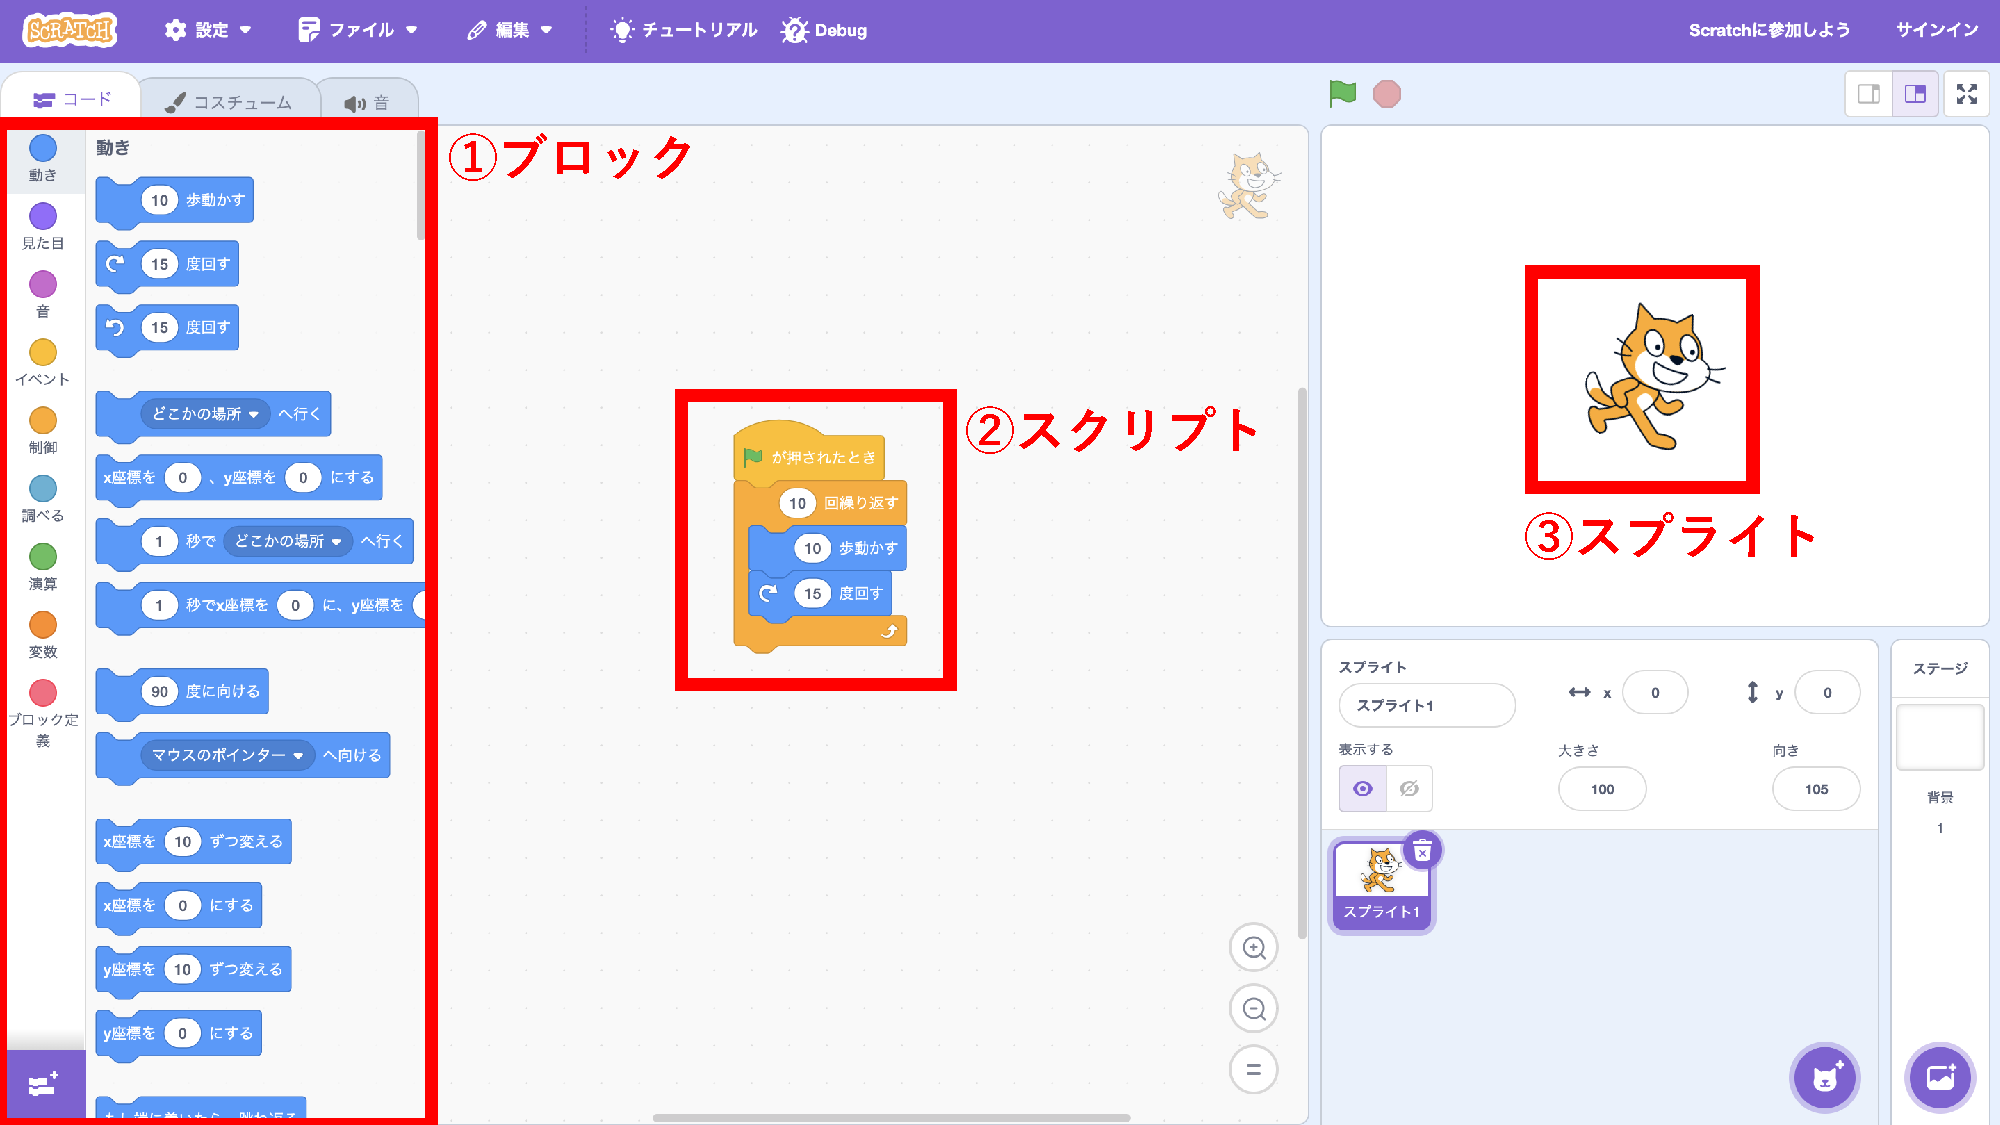
\includegraphics[width=0.8\linewidth]{@BSthesis2024_Horio/BSthesis2024_Horio_fig/scratch-edt.pdf}}
\caption{Scratch編集画面}
\label{fig:scratch-edt}
\end{figure}
%-------------------
%-------------------
\begin{table}[h]
    \centering
    \caption{ブロックの形状と性質}
    \label{Block}
    \renewcommand{\arraystretch}{1.2}
    \scalebox{1.0}{
    \begin{tabular}{c|c|c}
    \hline
    ブロックの形状 & 名前 & 性質
    \\ \hline
    \begin{minipage}{20mm}
      \centering
      \scalebox{0.5}{
\includegraphics{@BSthesis2024_Horio/BSthesis2024_Horio_fig/hatblock.png}}
    \end{minipage}
     & ハットブロック & スクリプトを開始するブロック
    \\ \hline
    \begin{minipage}{20mm}
      \centering
      \scalebox{2.0}{
\includegraphics{@BSthesis2024_Horio/BSthesis2024_Horio_fig/stackblock.png}}
    \end{minipage}
     & スタックブロック & 各種の命令を実行するブロック
    \\ \hline
    \begin{minipage}{20mm}
      \centering
      \scalebox{2.0}{
\includegraphics{@BSthesis2024_Horio/BSthesis2024_Horio_fig/tfblock.png}}
    \end{minipage}
     & 真偽ブロック & 真または偽のどちらかの状態を表すブロック
    \\ \hline
    \begin{minipage}{20mm}
      \centering
      \scalebox{0.5}{
\includegraphics{@BSthesis2024_Horio/BSthesis2024_Horio_fig/xblock.png}}
    \end{minipage}
     & 値ブロック & 数値や文字列を返すブロック
    \\ \hline
    \begin{minipage}{20mm}
      \centering
      \scalebox{0.5}{
\includegraphics{@BSthesis2024_Horio/BSthesis2024_Horio_fig/cblock.png}}
    \end{minipage}
     & C型ブロック & 間に挟まれたブロックを制御するブロック
    \\ \hline
    \begin{minipage}{20mm}
      \centering
      \scalebox{2.0}{
\includegraphics{@BSthesis2024_Horio/BSthesis2024_Horio_fig/capblock.png}}
    \end{minipage}
     & キャップブロック & スクリプトを停止するブロック
    \\ \hline
    \end{tabular}
    }
\end{table}
%-------------------
%-------------------
\begin{table}[h]
    \centering
    \caption{ブロックの色と性質}
    \label{Blockcolor}
    \scalebox{1.0}{
    \begin{tabular}{c|c|c}
    \hline
    ブロックの色 & 名前 & 性質
    \\ \hline
    \begin{minipage}{20mm}
      \centering
      \scalebox{0.5}{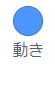
\includegraphics{@BSthesis2024_Horio/BSthesis2024_Horio_fig/move.png}}
    \end{minipage}
     & 動き & スプライトの動きを制御するブロック
    \\ \hline
    \begin{minipage}{20mm}
      \centering
      \scalebox{0.5}{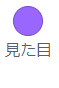
\includegraphics{@BSthesis2024_Horio/BSthesis2024_Horio_fig/look.png}}
    \end{minipage}
     & 見た目 & スプライトの見た目を制御するブロック
    \\ \hline
    \begin{minipage}{20mm}
      \centering
      \scalebox{0.5}{
\includegraphics{@BSthesis2024_Horio/BSthesis2024_Horio_fig/sound.png}}
    \end{minipage}
     & 音 & BGMやSEなどの音を制御するブロック
    \\ \hline
    \begin{minipage}{20mm}
      \centering
      \scalebox{0.5}{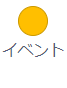
\includegraphics{@BSthesis2024_Horio/BSthesis2024_Horio_fig/event.png}}
    \end{minipage}
     & イベント & スクリプトを実行するトリガーを示すブロック
    \\ \hline
    \begin{minipage}{20mm}
      \centering
      \scalebox{0.5}{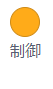
\includegraphics{@BSthesis2024_Horio/BSthesis2024_Horio_fig/seigyo.png}}
    \end{minipage}
     & 制御 & プログラムの処理の流れを制御するブロック
    \\ \hline
    \begin{minipage}{20mm}
      \centering
      \scalebox{0.5}{
\includegraphics{@BSthesis2024_Horio/BSthesis2024_Horio_fig/seach.png}}
    \end{minipage}
     & 調べる & スクリプトや操作の状態を調べるブロック
    \\ \hline
    \begin{minipage}{20mm}
      \centering
      \scalebox{0.5}{
\includegraphics{@BSthesis2024_Horio/BSthesis2024_Horio_fig/enzan.png}}
    \end{minipage}
     & 演算 & 演算を行うブロック
    \\ \hline
    \begin{minipage}{20mm}
      \centering
      \scalebox{0.5}{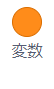
\includegraphics{@BSthesis2024_Horio/BSthesis2024_Horio_fig/hensu.png}}
    \end{minipage}
     & 変数 & 変数とリストを定義し,扱うブロック
    \\ \hline
    \begin{minipage}{20mm}
      \centering
      \scalebox{0.5}{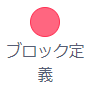
\includegraphics{@BSthesis2024_Horio/BSthesis2024_Horio_fig/teigi.png}}
    \end{minipage}
     & ブロック定義 & カスタムブロックを定義して使うことができるブロック
    \\ \hline
    \end{tabular}
    }
\end{table}
%-------------------
\section{Dr.Scratch}

Dr.ScratchとはMorenoらにより開発されたScratch作品のコンピュテーショナル・シンキング(CT)スキルを計測する支援ツールである\cite{moreno2015dr}.
Dr.Scratchでは,CTスキルを7概念の論理,制御フロー,同期,抽象化,データ表現,ユーザ対話性,並列処理に分類しており,各概念を0点から3点の合計21点で評価し,CTスコアと呼ぶ.CTスキルの各概念のスコア詳細は表\ref{CTscoreTable}に示す.また,CT習熟度がBasic,Developing,Masterの3区分に分類されており,0点から7点をBasic,8点から14点をDeveloping,15点から21点をMasterとしている.

図\ref{fig:scratch-edt}の作品をDr.Scratchを利用し,評価した場合,図\ref{fig:DrScratchgamen}のようになる.左側に合計スコア,CT習熟度が表示され,右側に,CTスキルの各概念で獲得することができたスコアが表示される.図\ref{fig:scratch-edt}の作品では,指定回数の繰り返しブロックを使用しているため,フロー制御が2点,緑の旗ブロックを使用しているため,ユーザ対話性が1点,オブジェクトのプロパティを編集しているため,データ表現が1点獲得している.

本研究では,Dr.ScratchによるScratch作品評価スコアのCTスコアを用いて,ユーザのCTスキルとリミックス作品の難易度を計測する.

%-------------------

\begin{table}[h]
    \centering
    \caption{CTスキルの概念\cite{橋谷直樹2022scratch}}
    \label{CTscoreTable}
    \scalebox{0.7}{
    \begin{tabular}{c|c|c|c|c}
    \hline
    CTスキルの概念 & 0点 & 1点 & 2点 & 3点
    \\ \hline
    抽象化 & - &
    \begin{tabular}{c}
    2つ以上の\\スクリプトを使用
    \end{tabular}
    & 定義ブロックを使用 & クローンブロックを使用
    \\ \hline
    並列 & - & 
    \begin{tabular}{c}
    緑の旗ブロックを\\2個以上使用 
    \end{tabular}
    & 
    \begin{tabular}{c}
    オブジェクトへのクリックにより\\2つ以上のスクリプトを\\同時に実行する機能を実装
    \end{tabular}
    & 
    \begin{tabular}{c}
    イベント動作により\\2つ以上のスクリプトを\\同時に実行する機能を実装
    \end{tabular}
    \\ \hline
    論理 & - & Ifブロックを使用 & If elseブロックを使用 & 論理演算ブロックを使用
    \\ \hline
    同期 & - & 待機ブロックを使用 &
    \begin{tabular}{c}
    メッセージ受信により\\プログラムを停止する機能を実装
    \end{tabular}
    &
    \begin{tabular}{c}
    指定条件を満たすまで\\プログラムを停止する処理を実装
    \end{tabular}
    \\ \hline
    フロー制御 & - &
    \begin{tabular}{c}
    2個以上の処理ブロックを\\連結して使用
    \end{tabular}
    &
    \begin{tabular}{c}
    指定回数/回数無制限の\\繰り返しブロックを使用
    \end{tabular}
    &
    \begin{tabular}{c}
    指定条件までの\\繰り返しブロックを使用
    \end{tabular}
    \\ \hline
    ユーザ対話性 & - & 緑の旗ブロックを使用 &
    \begin{tabular}{c}
    ユーザの入力を伴う\\ブロックを使用
    \end{tabular}
    &
    \begin{tabular}{c}
    マイクやビデオなどの\\作用を伴うブロックを使用
    \end{tabular}
    \\ \hline
    データ表現 & - &
    \begin{tabular}{c}
    オブジェクトの\\プロパティを編集
    \end{tabular}
    & 変数ブロックを使用 & リスト変数ブロックを使用
    \\ \hline
    \end{tabular}
    }
\end{table}

%-------------------
%-------------------
\begin{figure}[h]
\centerline{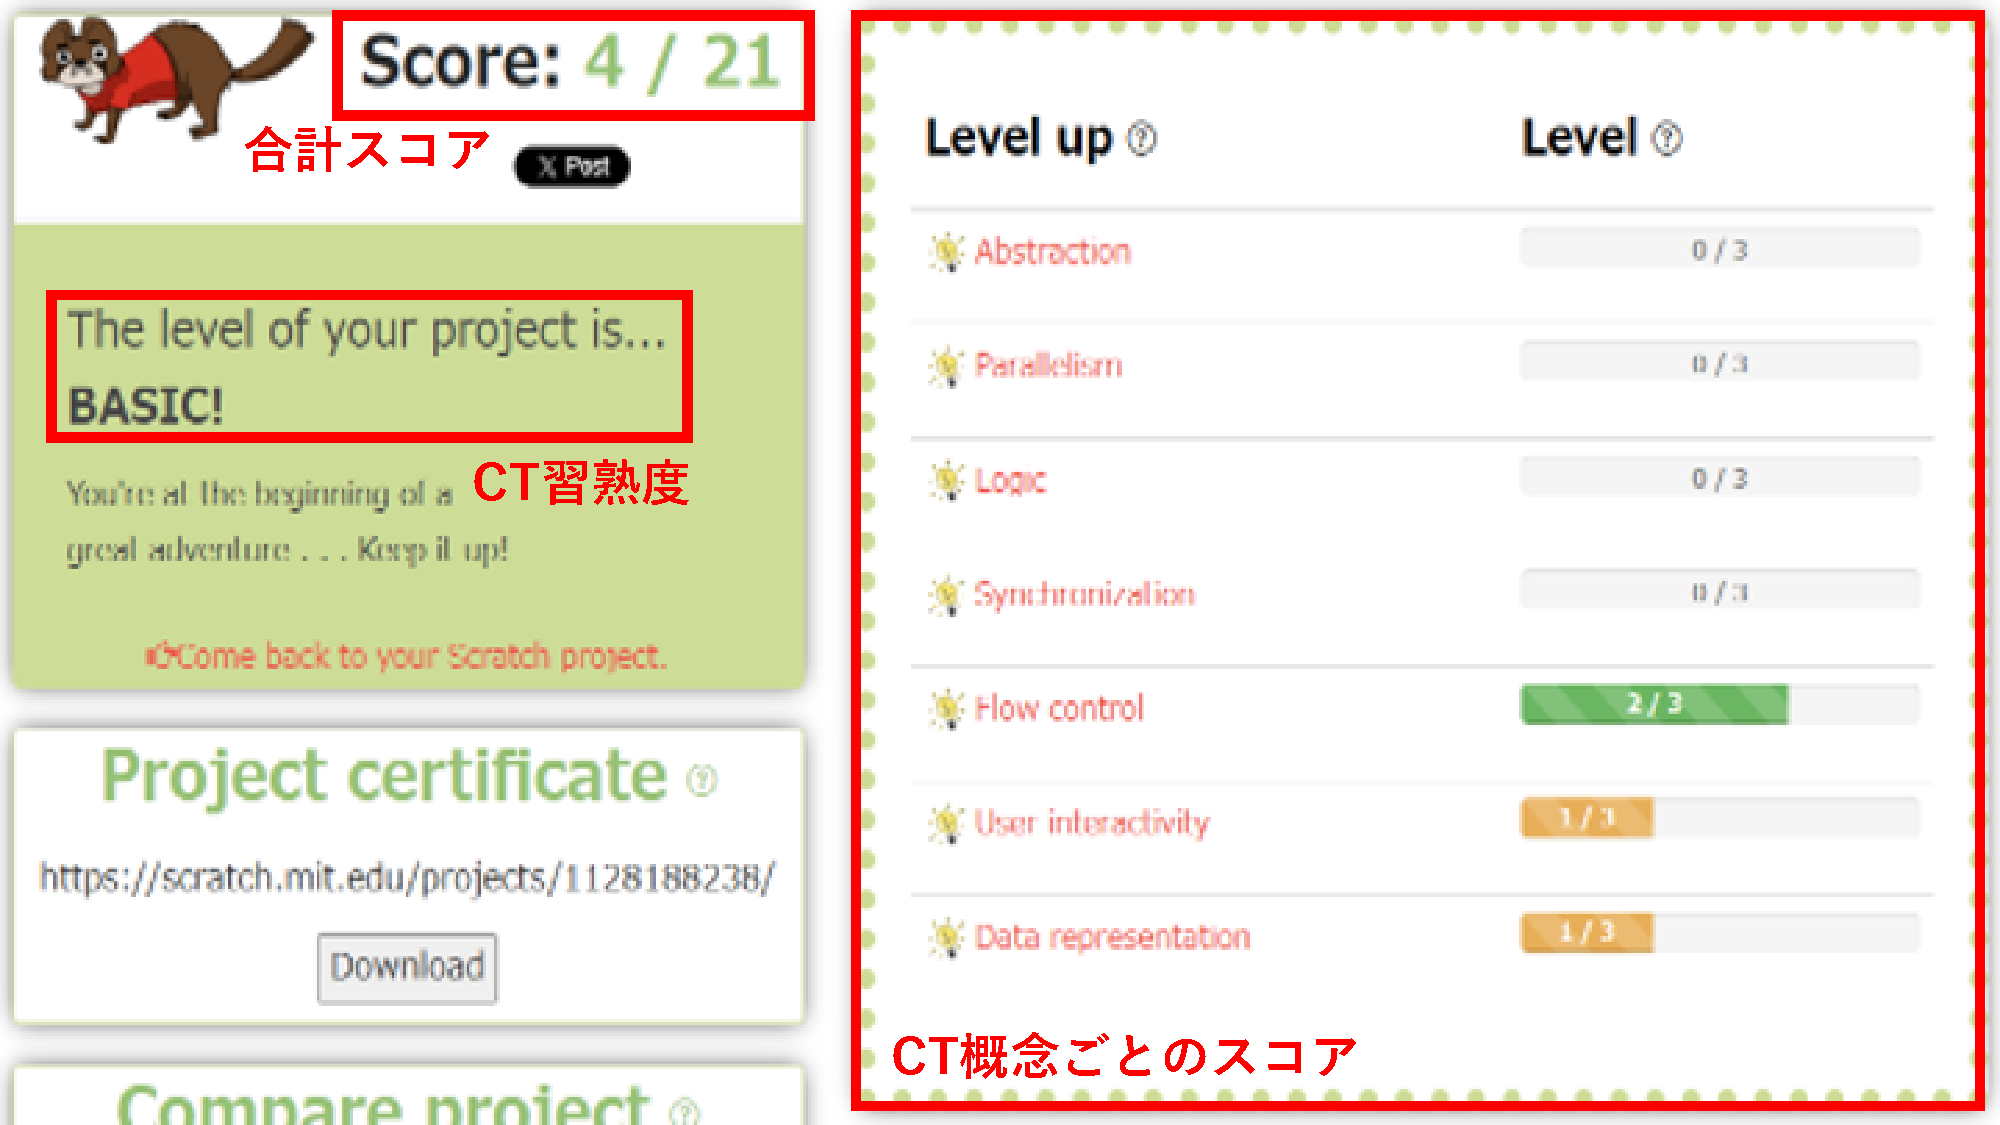
\includegraphics[width=1.0\linewidth]{@BSthesis2024_Horio/BSthesis2024_Horio_fig/DrScratchgamen.pdf}}
\caption{Dr.Scratchの評価画面}
\label{fig:DrScratchgamen}
\end{figure}
%-------------------


\section{従来研究}
Yangら\cite{10.1145/2724660.2724674}と橋谷ら\cite{橋谷直樹2022scratch}はリミックスがユーザのCTスキルにどのように影響するのかを調査し,リミックスすることで,CTスコアが向上すること,また,使用するブロックの種類数が増加することがわかった.しかし,必ず向上するわけでなく,リミックスを行うことで,CTスキルが向上したユーザの割合は示されておらず,リミックスがどのCTスキルのユーザに効果的なのかがわからない.

Fesakisらはリミックス元作品の協調性フィルタリングによるユーザ類似度でリミックス作品を推薦するという手法を提案した\cite{fesakis2009proposing}.
類似性を測定することができるJaccard係数を使用し,ユーザのリミックス元作品の一致不一致に重みづけを行い,多次元尺度構成法を用いることで類似関係を視覚化し,類似しているユーザを見つけ出した.
例えば,ユーザAとユーザBが類似しているとすると,ユーザAがリミックスした作品かつ,ユーザBがリミックスしたことのない作品をユーザBに推薦する手法である.
リミックスを行うことによるCTスキル向上にユーザのCTスキルが大きく関係しているならば,従来手法は非常に効果的だと考える.しかし,従来手法では,類似したユーザがいない場合に推薦することが不可能であることと,CTスキル向上に寄与しない作品まで推薦することが考えられる.


\section{動機}
近年,日本では2020年度から小学校のプログラミング教育の必修化,2021年度から中学校の技術分野において,プログラミングに関する内容の充実,2022年度から高等学校の情報科において,共通必履修科目「情報1」の新設がされた\cite{monkashou}.しかし,指導者の情報不足や人材不足,予算不足による指導者に対する問題が複数挙げられた\cite{monkashou2}.

また,従来研究によりScratchにおけるリミックスが,ユーザのCTスキル向上に有効だと示された.極端な難易度のものをリミックスしてもCTスキルへの効果が少なく,ユーザのCTスキルに寄与したものは,ユーザのCTスキルに適した難易度の作品のリミックスだと考える.しかし,現在のScratchでは作品を探す手段はキーワード検索のみであり,ユーザのCTスキルに適した作品を探すことは困難である.

指導者不足の問題とScratchにおける作品検索問題を解決する有効な手段として,Scratchにおけるリミックス元作品の推薦が挙げられる.指導者不足の問題は,プログラミング教育の自動化を進めることが解決に有効であり,自動化の1つとしてScratchにおける推薦機能が挙げられる.ユーザがCTスキルを向上させるために,ユーザのCTスキルに適したカリキュラムの準備や参考作品の準備,採点をする必要がなく,学習を進めることが可能になる.推薦のためにはユーザのCTスキル向上に有効な作品の情報と基準が求められる.そこで本研究では,Scratchのリミックス機能におけるユーザのCTスキルに適した作品推薦に向けて,ユーザのCTスキルとリミックス作品の関係について分析を行う.

\section{リサーチクエスチョン}

以下のRQの目的について説明をする.
\begin{itemize}
  \item\textbf{RQ1:CTスコアは他ユーザの作品をリミックスすることによって向上するか?}
  \item\textbf{RQ2:リミックスにより向上しやすいCTスキルの概念は異なるか?}
  \item\textbf{RQ3:CTスコアによって,向上しやすいCTスキルの概念は異なるか?}
\end{itemize}

RQ1の目的として,リミックスがどのCTスコアのユーザにも有効かを調査するために,リミックス元作品とリミックス前後の作品のCTスコアを分析する.
RQ2の目的として,RQ1ではCTスコアにより分析を行ったが,同じCTスコアでも獲得しているCTスキルの概念のスコアは異なるため,CTスキルの概念ごとに着目し,リミックス元作品とリミックス前後の作品を分析する.
RQ3ではCTスキルの概念同士に相関関係があるかを調査するために,リミックスによるCTスキルの各概念の向上をCTスコアに基づいて視覚化し,分析を行う.

詳細については4章,5章,6章で述べる.

\chapter{ケーススタディ}

\section{概要}
本研究では,ユーザのCTスキルとリミックス作品の関係を分析するため,リミックス前作品,リミックス元作品,リミックス作品,リミックス後作品を重視する.以下で,各作品の定義を詳しく述べる.
\begin{itemize}
  \item リミックス前作品
  
  対象のリミックス作品より前に制作したオリジナル作品のうち,獲得したCTスコアが最も高い作品.
  
  \item リミックス元作品
  
  対象のリミックス作品のリミックスを行う前の状態の作品.
  
  \item リミックス作品
  
  対象のリミックス作品.

  \item リミックス後作品
  
  対象のリミックス作品より後に制作した直近のオリジナル作品3件以下のうち,獲得したCTスコアが最も高い作品.3件以下とした理由は,オリジナル作品の制作を重ねることによるCTスコア向上の影響を軽減するためである.

\begin{figure}[h]
\centerline{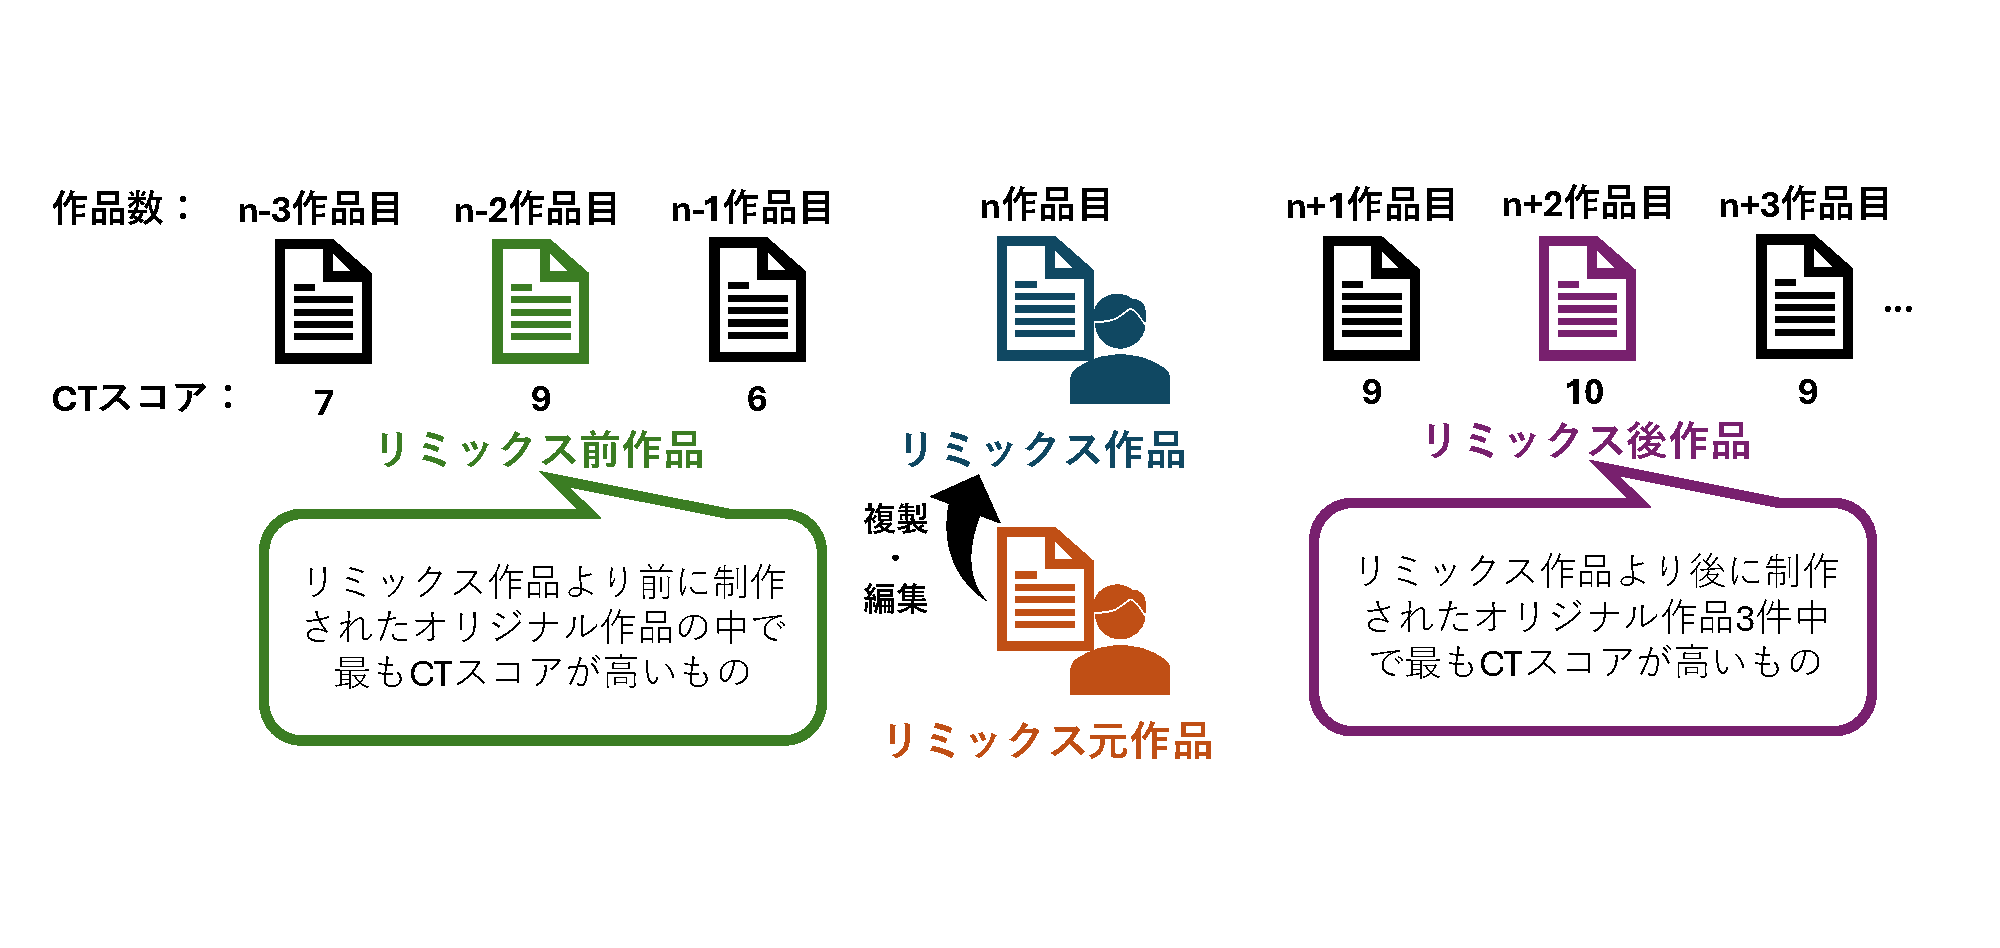
\includegraphics[width=0.9\linewidth]{@BSthesis2024_Horio/BSthesis2024_Horio_fig/case.pdf}}
\caption{リミックス前,リミックス元作品,リミックス作品,リミックス後作品の定義}
\label{fig:case}
\end{figure}
%-------------------
  
\end{itemize}
リミックス前作品,リミックス元作品,リミックス作品,リミックス後作品のそれぞれの作品のCTスコアを元に,議論を進める.

\section{データセット}
本研究ではScratch上に公開されているScratch3.0以降の作品のjsonデータをScratchAPI\footnote{\url{https://ja.scratch-wiki.info/wiki/Scratch_API_(2.0)}}により収集した.各作品のjsonデータには,作者ID,作品ID,リミックス元作品ID,スクリプトの情報などが含まれている.作品IDの昇順が制作された作品の順番となっている.本研究では,作者IDによりリミックス前作品,リミックス作品,リミックス後作品の一致,作品IDにより作品制作順の取得,リミックス元作品IDの有無によりリミックス作品の決定,リミックス元作品の取得,スクリプトの情報により使用しているブロック,スプライトの取得を行っている.

オリジナル作品,リミックス作品を含め,20作品以上制作したことがあり,リミックスを行ったことがあるユーザを対象とし,データセットの収集を行う.これにより,合計7,551人のユーザの136,283件の作品が本研究の分析の対象となった.その中に,オリジナル作品は89,226件,リミックス作品は47,057件含む.また,リミックス作品について,リミックス元作品のデータ取得も行った.リミックス元作品がScratch3.0以前のものや,非公開になっているものがあり,取得できないリミックス元作品を除いて,取得することができたリミックス元作品は22,271件ある.
% %-------------------
% \begin{table}[t]
%     \centering
%     \caption{各データセットの数}
%     \label{CTscoreTable}
%     \scalebox{1.0}{
%     \begin{tabular}{c|c}
%     \hline
%     データセット & 件数
%     \\ \hline
%     オリジナル作品 & 89,226
%     \\ \hline
%     リミックス作品 & 47,057
%     \\ \hline
%     リミックス元作品 & 22,271
%     \\ \hline
%     \end{tabular}
%     }
% \end{table}
% %-------------------
\chapter{RQ1:ユーザのCTスコアは、他ユーザの作品をリミックスすることによって向上するか?}

\section{概要}
RQ1ではリミックスすることで,ユーザのCTスコアが向上しているかを調査する.従来研究により,リミックスを行うことで,CTスコアが向上することは示されたが,必ず向上するわけでなく,実際に向上しているユーザの割合は示されていない.また,リミックスのみの影響ではなく,オリジナル作品の制作を重ねることで向上している可能性がある.そのため,リミックスを行うことで,CTスコアが向上しているか,不変か,低下しているかをリミックス前のCTスコアごとに調査する.

\section{分析手法}
分析手法として,箱ひげ図とヒストグラムにより視覚化を行う.使用するデータは,データセットのリミックス前作品,リミックス元作品,リミックス後作品である.

箱ひげ図では,縦軸をリミックス前作品のCTスコアとリミックス元作品のCTスコアの差とし,横軸をリミックス前作品のCTスコアとする.横軸では,リミックス前作品のCTスコアごとにリミックス前作品のCTスコアとリミックス後作品のCTスコアを比較し,向上したユーザ,不変のユーザ,低下したユーザの3つを出力する.

ヒストグラムでは,縦軸をユーザ数とし,横軸をリミックス前作品のCTスコアとする.横軸では,リミックス前作品のCTスコアごとにリミックス前作品のCTスコアとリミックス後作品のCTスコアを比較し,向上したユーザ,不変のユーザ,低下したユーザの3つを出力する.

検定として,CTスコアが向上したユーザと低下したユーザの2群に対し,マン・ホイットニーのU検定を用い,有意差を算出する.有意水準は0.05とする.

\section{分析結果}
図\ref{fig:rq1-CTscore}はリミックスによるCTスコアへの影響を示した箱ひげ図と各箱ひげ図のユーザ数を示したヒストグラムの結果である.

CTスコアが向上したユーザと低下したユーザの2群に対するマン・ホイットニーのU検定ではp値<0.05であったため,図\ref{fig:rq1-CTscore}の各スコアの向上したユーザと低下したユーザの2群には統計的に有意な差がある.

%-------------------
\begin{figure}[h]
\centerline{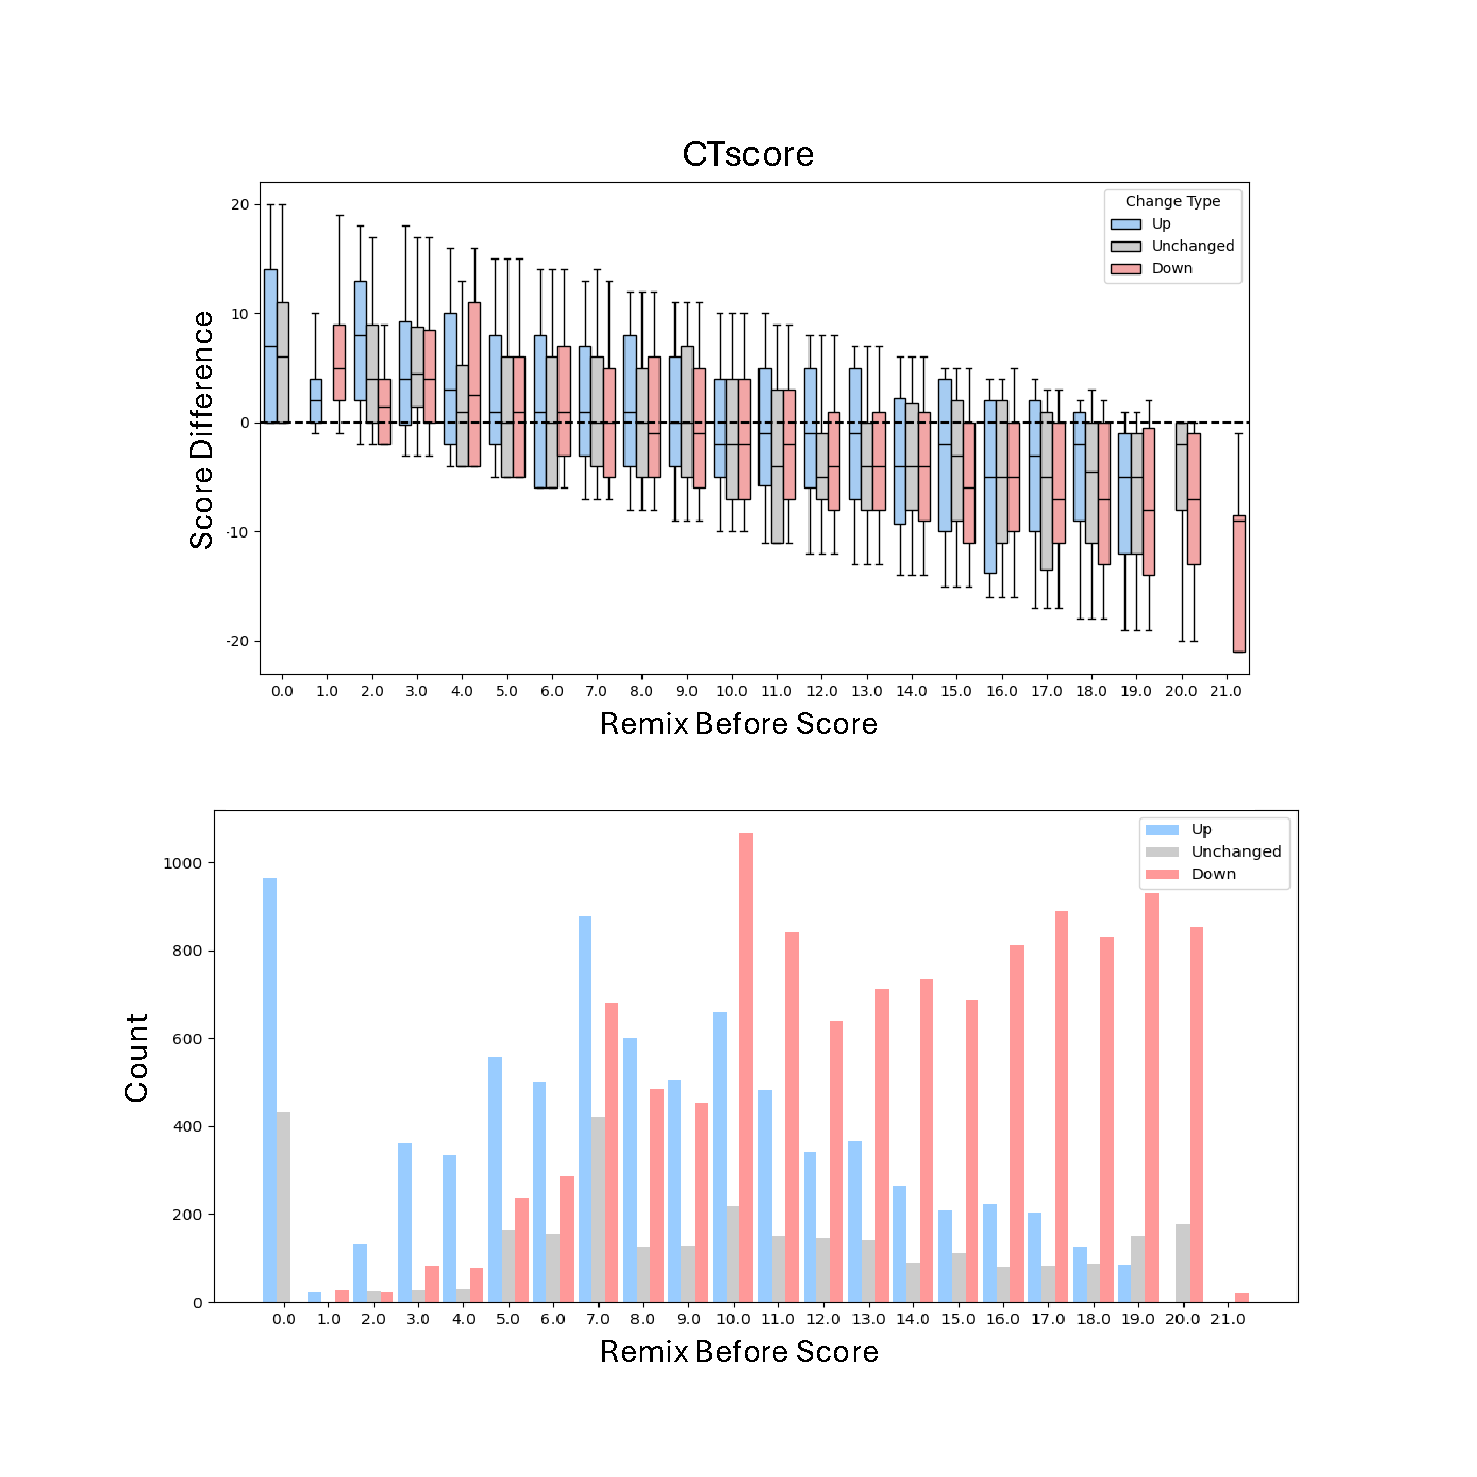
\includegraphics[width=0.9\linewidth]{@BSthesis2024_Horio/BSthesis2024_Horio_fig/rq1-CTscore.pdf}}
\caption{リミックスによるCTスコア変化}
\label{fig:rq1-CTscore}
\end{figure}
%-------------------

\section{考察}
ヒストグラムに着目すると,9点以下はCTスコアが向上したユーザ数が低下したユーザ数を上回っており,10点以上は低下したユーザ数が向上したユーザ数を上回っている.このことからリミックスはCTスコアが9点以下のユーザに対し有効であり,10点以上のユーザに対してはあまり効果が得られない.CTスコアを向上させるために,9点以下のユーザは獲得が容易なCTスキルの概念を向上させており,10点以上のユーザは獲得が困難なCTスキルの概念の向上が必要となっていることが考えられる.

箱ひげ図に着目すると,CTスコアが向上した多くのユーザが低下したユーザに比べてCTスコアが高い作品をリミックスしているが,向上したユーザが低下したユーザに比べてCTスコアが低い作品をリミックスしている場合もある.このことから,リミックス元作品のCTスコアとユーザのCTスコアの差はCTスコア向上に大きな影響を与えず,どの作品をリミックスしても効果が得られると考えられる.

\chapter{RQ2:リミックスにより向上しやすいCTスキルの概念は異なるか?}
\section{概要}
RQ2では,CTスキルの各概念に着目し,ユーザのCTスキルの概念が向上しているかを調査する.RQ1ではCTスコアごとに着目したが,CTスコアでは,同じスコアを獲得していても,CTスキルの各概念のスコアは異なる.そのため,リミックスを行うことで,CTスキルの概念が向上しているか,不変か,低下しているかをリミックス前作品のCTスキルの概念のスコアごとに調査する.

\section{分析手法}
分析手法として,CTスキルの各概念でRQ1と同様に箱ひげ図とヒストグラムにより視覚化を行う.使用するデータは,データセットのリミックス前作品,リミックス元作品,リミックス後作品である.

箱ひげ図では,縦軸をリミックス前作品とリミックス元作品のCTスキルの各概念のスコアの差とし,横軸をリミックス前作品のCTスキルの各概念のスコアとする.横軸では,リミックス前作品のCTスキルの概念のスコアごとに,リミックス前作品とリミックス後作品のCTスキルの概念のスコアを比較し,向上したユーザ,不変のユーザ,低下したユーザの3つを出力する.

ヒストグラムでは,縦軸をユーザ数とし,横軸をリミックス前作品のCTスキルの各概念のスコアとする.横軸では,リミックス前作品のCTスキルの概念のスコアごとに,リミックス前作品とリミックス後作品のCTスキルの概念のスコアを比較し,向上したユーザ,不変のユーザ,低下したユーザの3つを出力する.

検定として,各箱ひげ図のCTスキルの概念のスコアが向上したユーザと低下したユーザの2群に対し,マン・ホイットニーのU検定を用い,有意差を算出する.有意水準は0.05とする.

\section{分析結果}
図\ref{fig:rq2-1},図\ref{fig:rq2-2}はCTスキルの概念ごとにリミックスによるCTスキルの概念への影響を示した箱ひげ図と箱ひげ図のユーザ数を示したヒストグラムの結果である.

CTスキルの概念のスコアが向上したユーザと低下したユーザの2群に対するマン・ホイットニーのU検定では図\ref{fig:rq2-1},図\ref{fig:rq2-2}の全ての箱ひげ図においてp値<0.05であったため,図\ref{fig:rq2-1},図\ref{fig:rq2-2}の各箱ひげ図のCTスキルの概念のスコアが向上したユーザと低下したユーザの2群には統計的に有意な差がある.


%-------------------
\begin{figure}[h]
\centerline{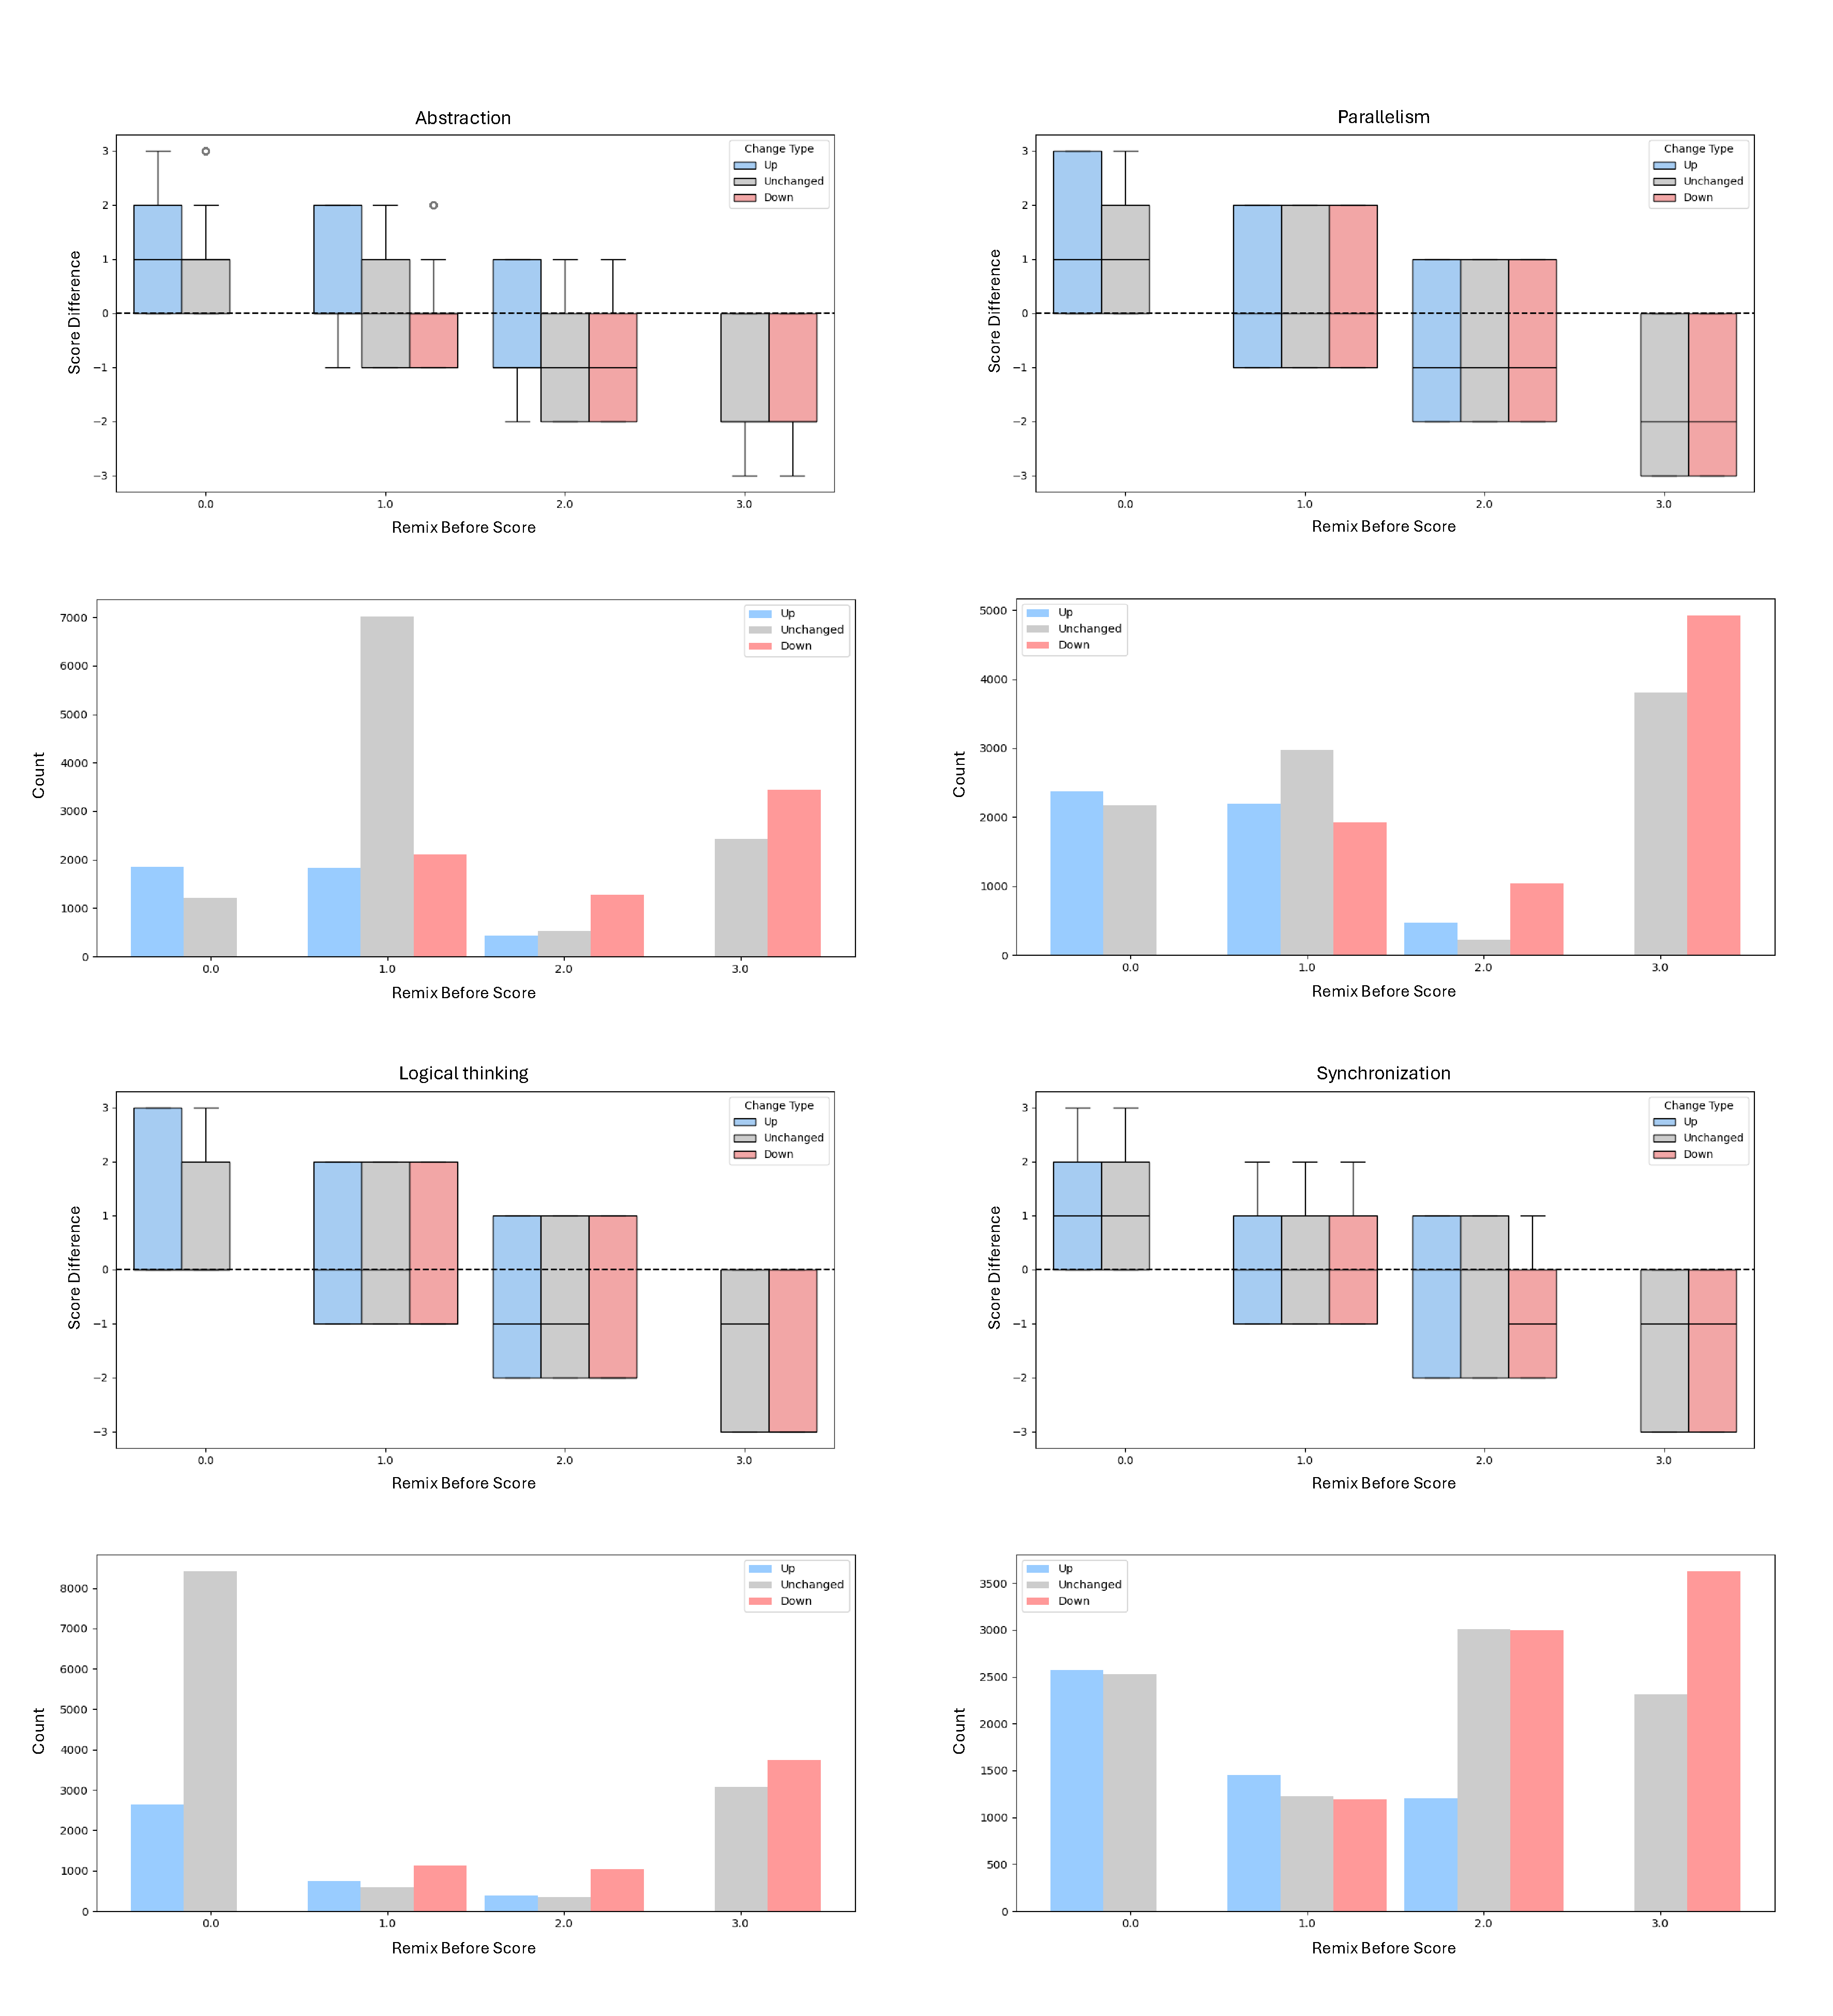
\includegraphics[width=1.2\linewidth]{@BSthesis2024_Horio/BSthesis2024_Horio_fig/rq2-1.pdf}}
\caption{リミックスによるCTスキルの概念のスコア変化-1}
\label{fig:rq2-1}
\end{figure}
%-------------------

%-------------------
\begin{figure}[h]
\centerline{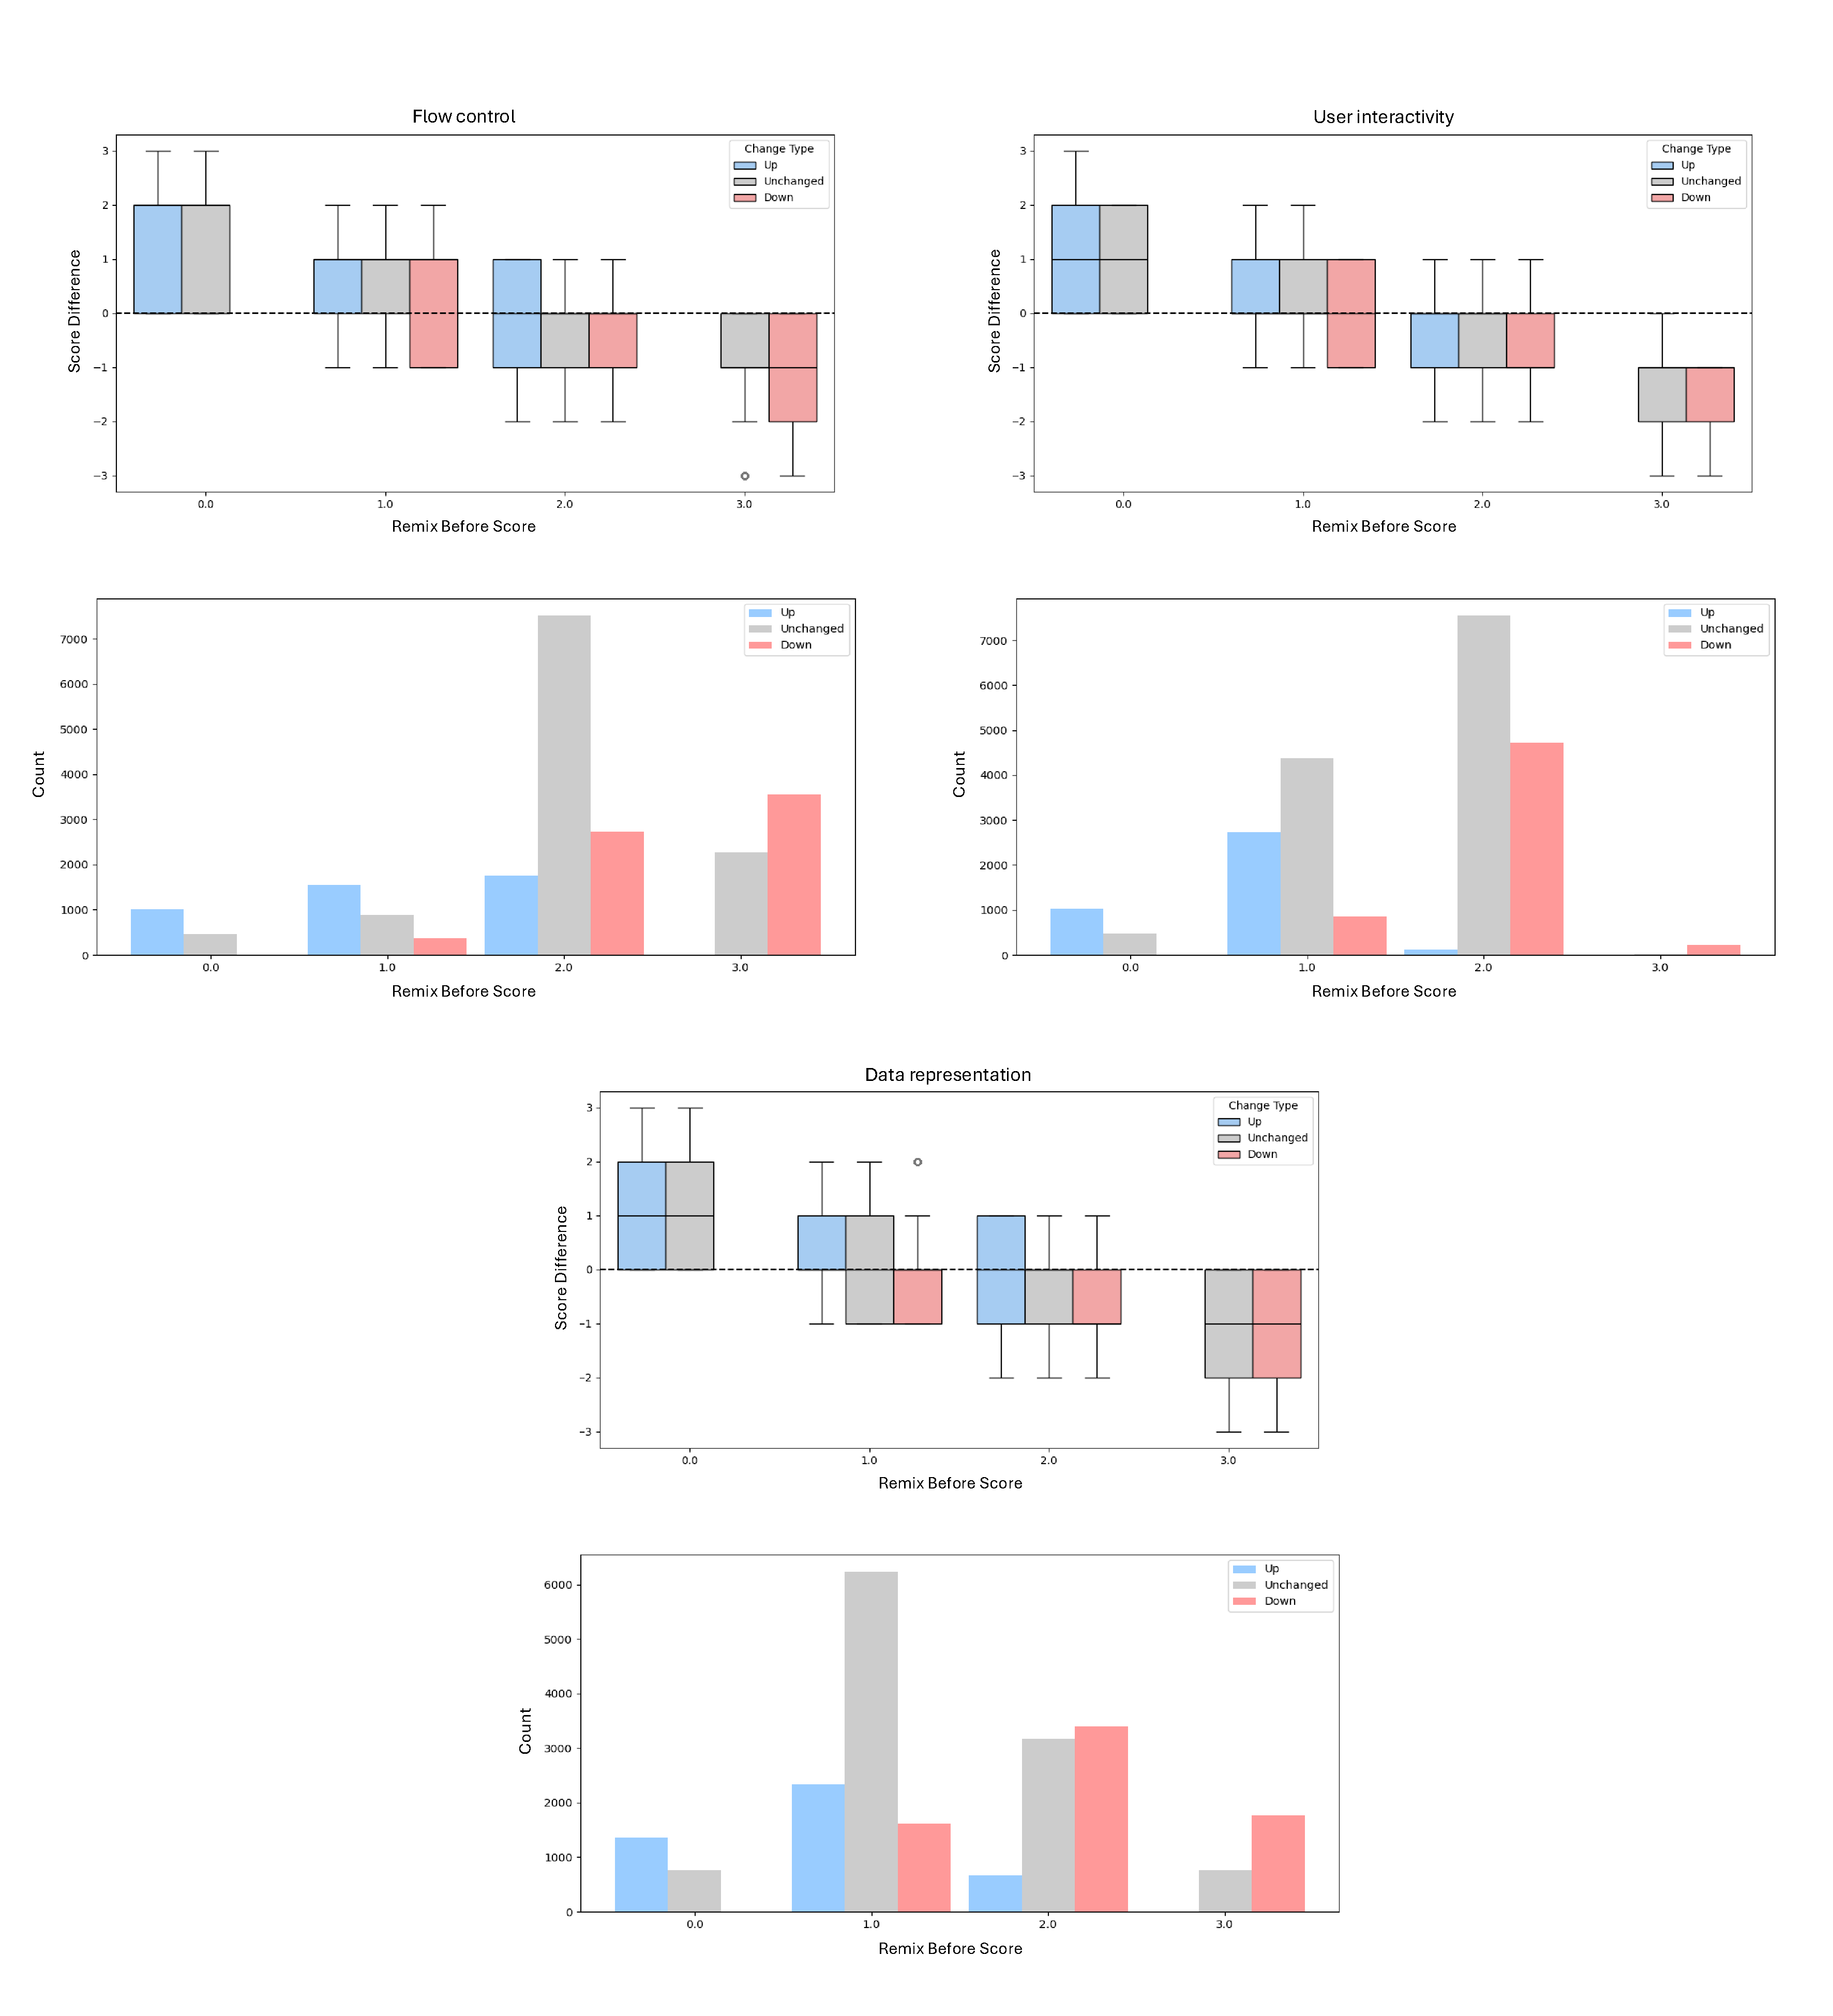
\includegraphics[width=1.2\linewidth]{@BSthesis2024_Horio/BSthesis2024_Horio_fig/rq2-2.pdf}}
\caption{リミックスによるCTスキルの概念のスコア変化-2}
\label{fig:rq2-2}
\end{figure}
%-------------------

\section{考察}
ヒストグラムに着目する.
抽象化や並列,論理ではスコアごとの向上したユーザ数と低下したユーザ数に大きな差はない.そのため,リミックスにより効果が得られることは確実ではない.
また,同期ではリミックス前作品のスコアが2点のユーザがリミックスをすると,低下したユーザ数が向上したユーザ数を大幅に上回っており,2点以上でリミックスによる効果が得られにくい.
フロー制御やユーザ対話性,データ表現では,いずれもリミックス前作品のスコアが1点では向上したユーザ数が低下したユーザ数に比べて多く,2点では低下したユーザ数が向上したユーザ数に比べて多くなっている.このことから,フロー制御やユーザ対話性,データ表現が1点以下のユーザはリミックスにより効果が得られやすく,2点以上のユーザは効果が得られにくい.

箱ひげ図に着目する.
並列や論理では,向上したユーザと低下したユーザのリミックス元作品のスコアに差がほとんどない.このことから,リミックス元作品の並列や論理のスコアとユーザのスコアの差はスコア向上に大きな影響を与えず,どの作品をリミックスしても効果が得られる可能性がある.
CTスキルの概念のスコアが向上したユーザと低下したユーザのリミックス元作品のスコアに差があるものとして.抽象化,データ表現が挙げられる.抽象化,データ表現のスコアが向上したユーザは低下したユーザに比べて,リミックス元作品のスコアが高い.このことから,抽象化,データ表現を向上させたいユーザは,抽象化,データ表現のスコアがユーザより高い作品をリミックスすると効果が得られる.特に,データ表現では,ヒストグラムにより,1点以下のユーザがユーザのスコアより高い作品をリミックスをすることで効果が得られやすい.
ユーザ対話性では,リミックス前作品が1点以下の,スコアが向上したユーザは低下したユーザに比べてスコアが高い作品をリミックスしている.また,ヒストグラムにより,ユーザ対話性はリミックス前作品が1点以下のユーザは,リミックスの効果を得られやすい.これより,ユーザ対話性が1点以下であり,向上させたいユーザはユーザ対話性のスコアがユーザより高い作品をリミックスすると効果が得られやすい.

リミックスによって向上しやすいCTスキルの概念が異なるだけでなく,CTスキルの各概念のスコアによっても,向上のしやすさに違いがあることがわかる.



\chapter{RQ3:CTスコアによって,向上しやすいCTスキルの概念は異なるか?}
\section{概要}
RQ2で,CTスキルの各概念に対するリミックスの影響について調査をした.RQ3では,CTスコアによってCTスキルの各概念の獲得のしやすさが異なるかを調査する.ある1つのCTスキルの概念のみが向上するわけではなく,CTスキルの各概念同士に相関関係があると考える.そのため,CTスコアに基づいてCTスキルの各概念の向上を視覚化し,分析する.

\section{分析手法}
分析手法として,RQ1,RQ2と同様に箱ひげ図とヒストグラムにより視覚化を行う.使用するデータはデータセットのリミックス前作品,リミックス元作品,リミックス後作品である.

箱ひげ図では,縦軸をリミックス前作品のCTスコアとリミックス元作品のCTスコアの差とし,横軸をリミックス前作品のCTスコアとする.横軸では,リミックス前作品のCTスコアごとに,リミックス前作品とリミックス後作品のCTスキルの概念のスコアを比較し,向上したユーザ,不変のユーザ,低下したユーザの3つを出力する.

ヒストグラムでは,縦軸をユーザ数とし,横軸をリミックス前作品のCTスコアとする.横軸では,リミックス前作品のCTスコアごとに,リミックス前作品とリミックス後作品のCTスキルの概念のスコアを比較し,向上したユーザ,不変のユーザ,低下したユーザの3つを出力する.

検定として,各箱ひげ図のCTスキルの概念のスコアが向上したユーザと低下したユーザの2群に対し,マン・ホイットニーのU検定を用い,有意差を算出する.有意水準は0.05とする.

\section{分析結果}
図\ref{fig:rq3-1},図\ref{fig:rq3-2}はリミックスによるCTスコアに基づいたCTスキルの概念への影響を示した箱ひげ図と箱ひげ図のユーザ数を示したヒストグラムの結果である.

CTスキルの概念のスコアが向上したユーザと低下したユーザの2群に対するマン・ホイットニーのU検定では図\ref{fig:rq3-1},図\ref{fig:rq3-2}の全ての箱ひげ図においてp値<0.05であったため,図\ref{fig:rq3-1},図\ref{fig:rq3-2}の各箱ひげ図のCTスキルの概念のスコアが向上したユーザと低下したユーザの2群には統計的に有意な差がある.

%-------------------
\begin{figure}[h]
\centerline{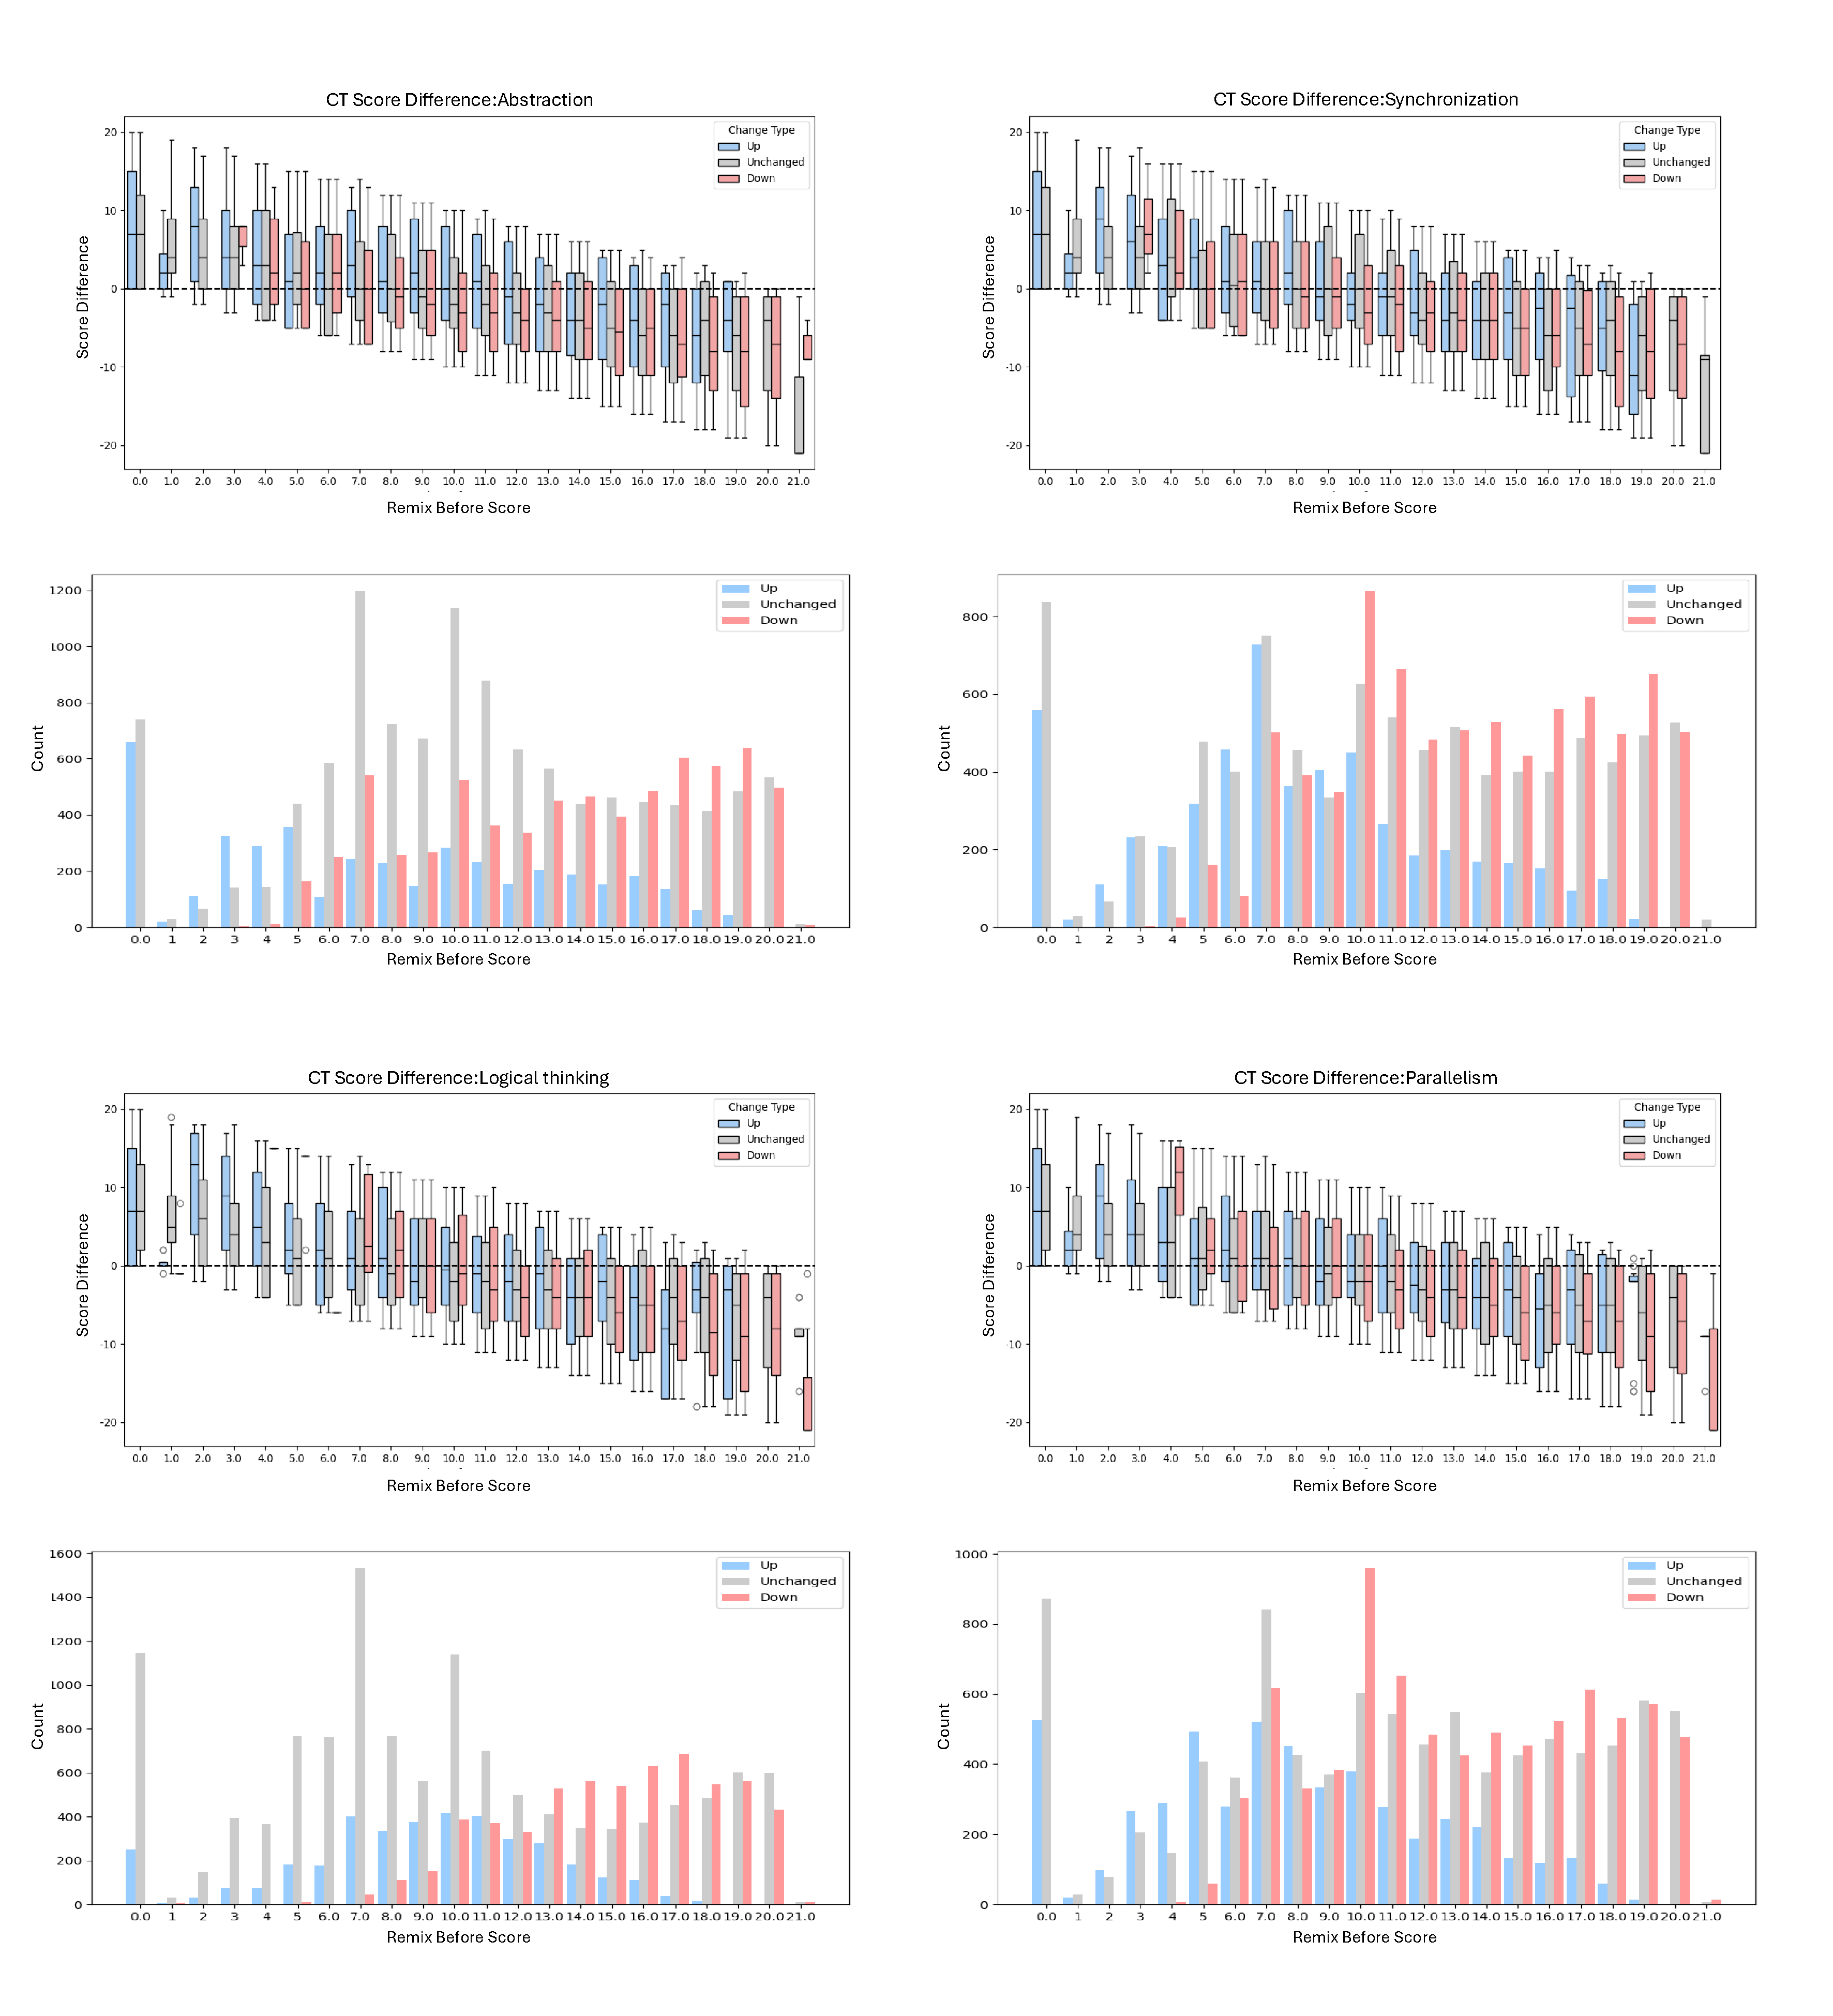
\includegraphics[width=1.2\linewidth]{@BSthesis2024_Horio/BSthesis2024_Horio_fig/rq3-1.pdf}}
\caption{リミックスによるCTスコアに基づいたCTスキルの概念のスコア変化-1}
\label{fig:rq3-1}
\end{figure}
%-------------------

%-------------------
\begin{figure}[h]
\centerline{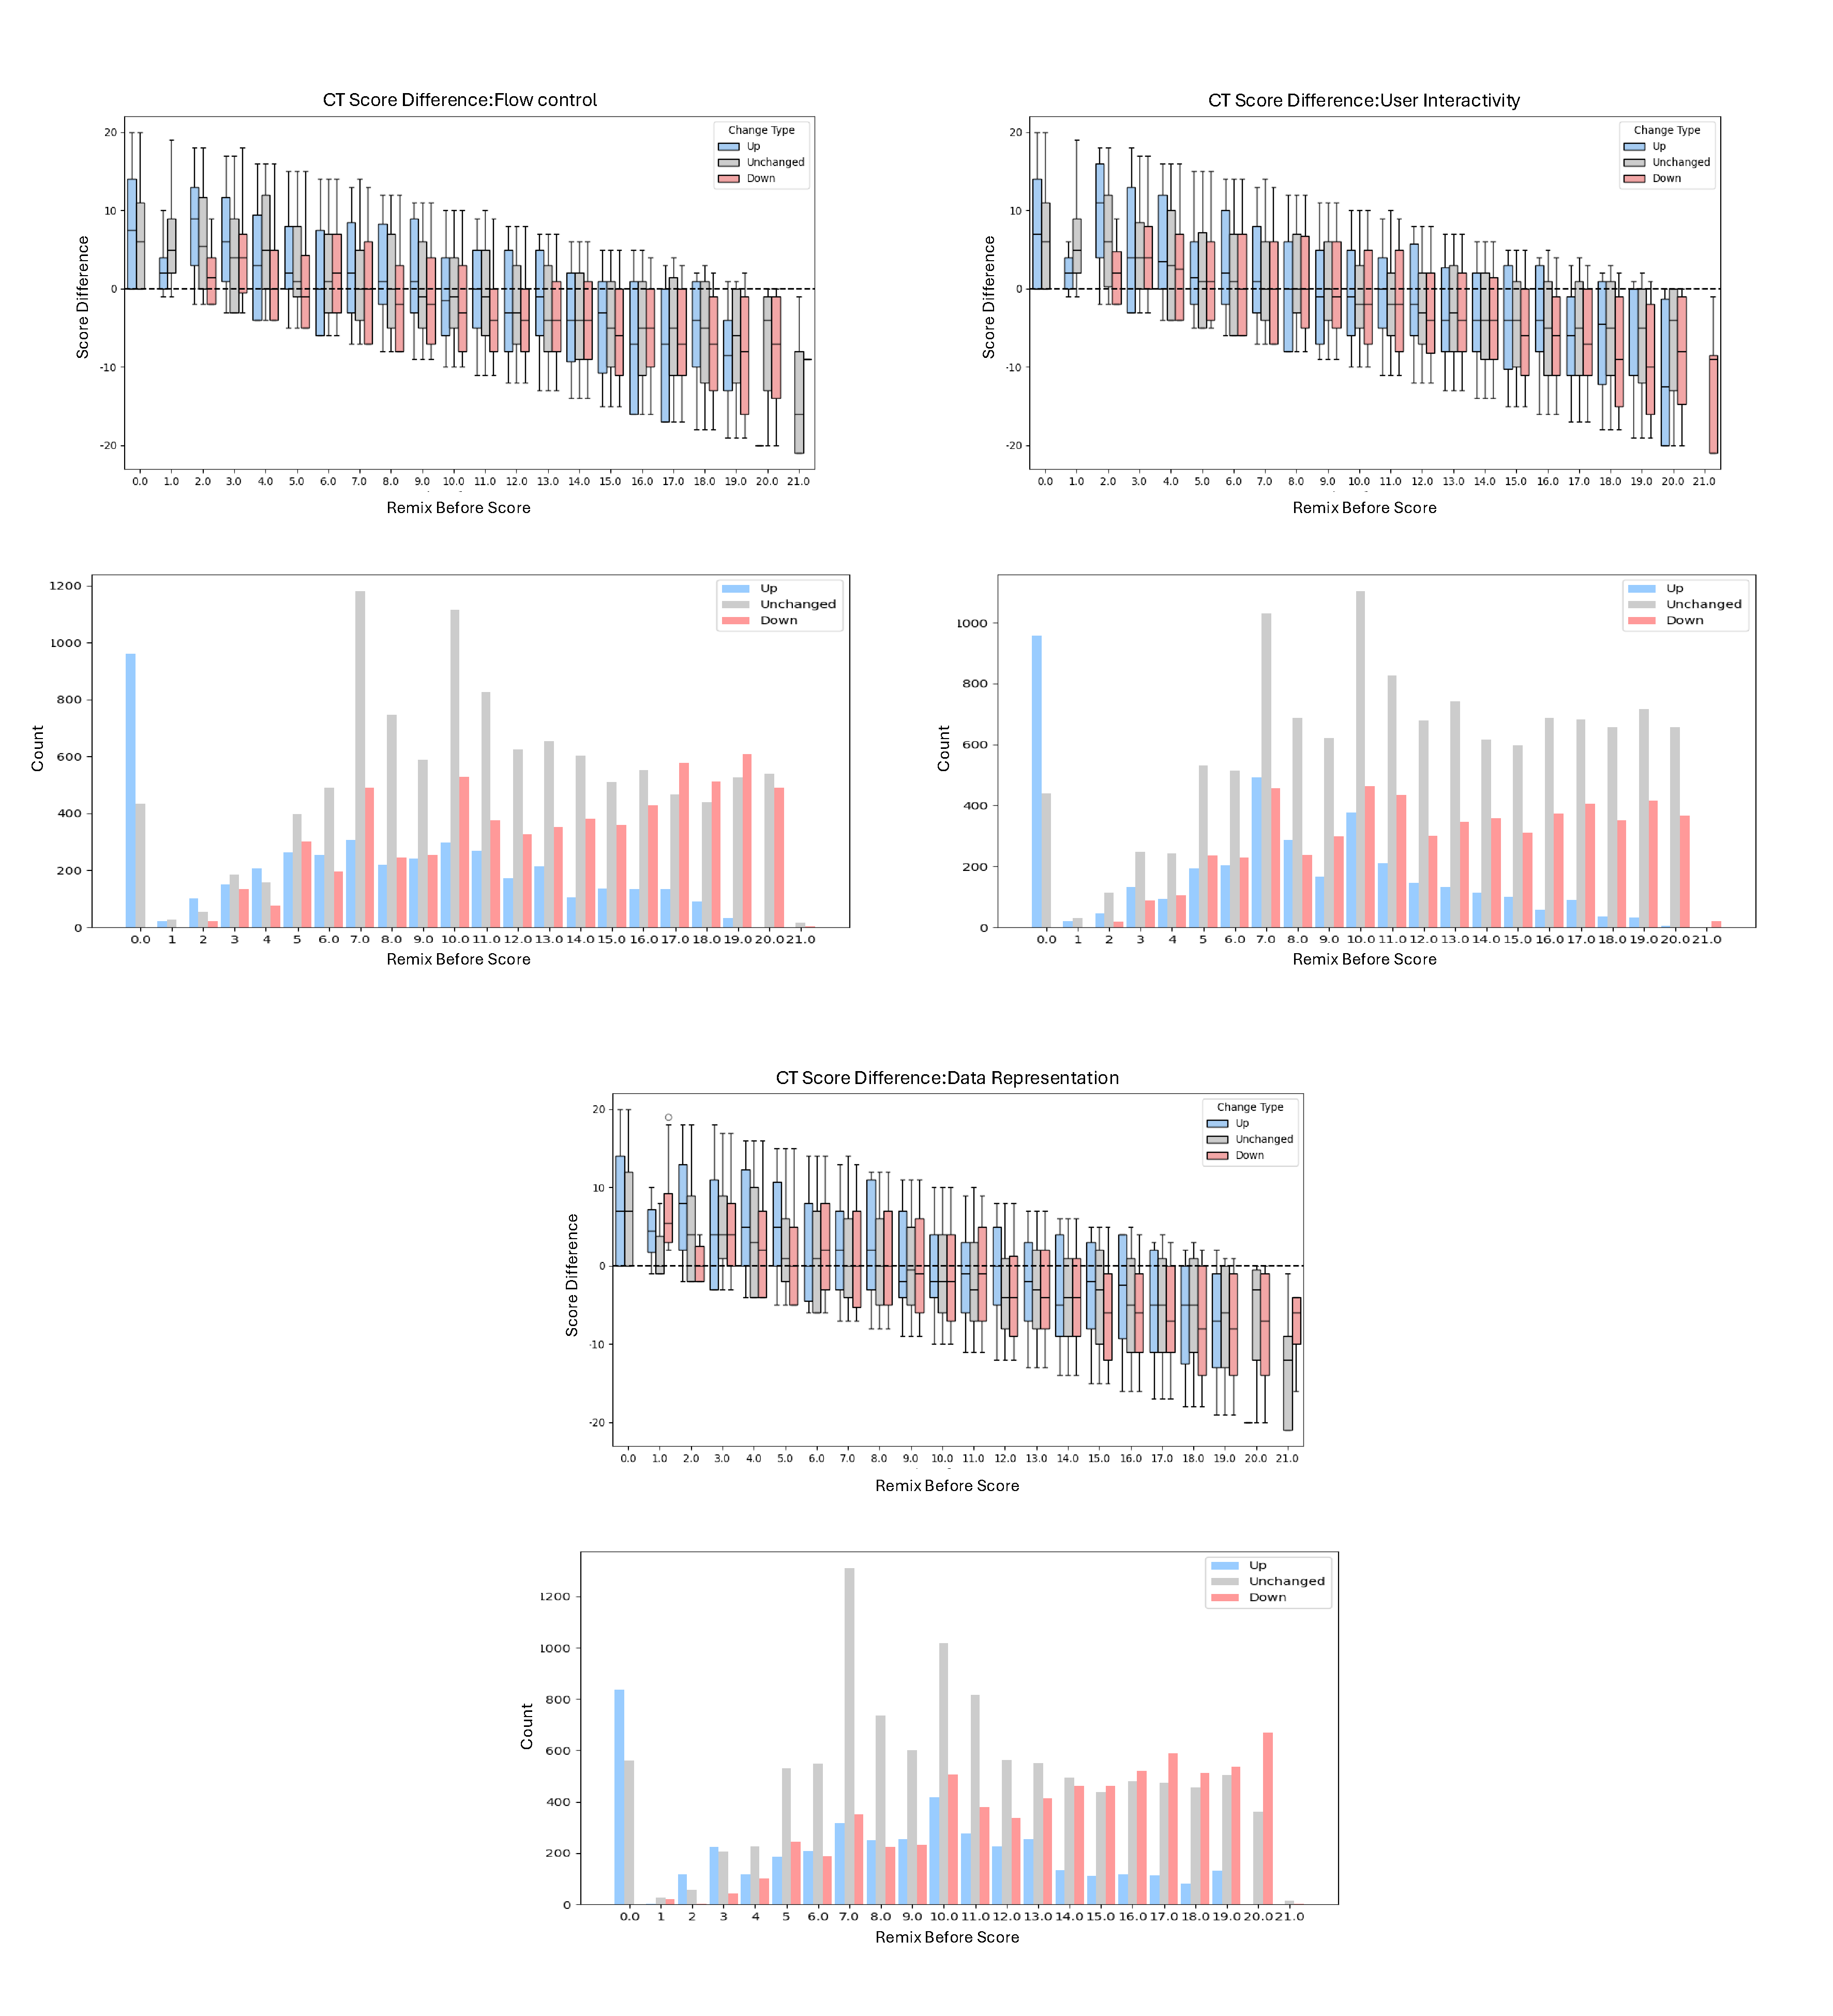
\includegraphics[width=1.2\linewidth]{@BSthesis2024_Horio/BSthesis2024_Horio_fig/rq3-2.pdf}}
\caption{リミックスによるCTスコアに基づいたCTスキルの概念のスコア変化-2}
\label{fig:rq3-2}
\end{figure}
%-------------------

\section{考察}
ヒストグラムに着目する.どのCTスキルの概念のヒストグラムにおいても,リミックス前のCTスコアが低いほど,CTスキルの概念が向上したユーザが多く,リミックス前のCTスコアが高いほど,CTスキルの概念が低下したユーザが多い.これは,CTスコアが低いときに獲得しやすいCTスキルの概念を獲得し,CTスコアが高くなると獲得が困難なCTスキルの概念を獲得する必要が出てくるからであると考える.

箱ひげ図に着目すると,抽象化とフロー制御のスコアが向上したユーザは低下したユーザに比べ,CTスコアが高い作品をリミックスしており,CTスコアの影響が大きい可能性がある.抽象化とフロー制御に着目して,議論を進める.
抽象化のリミックス前作品のCTスコアが6,7,8点に着目する.CTスコアが6,7点で抽象化のスコアが向上したユーザ数が低下したユーザ数に比べて大幅に下回っているが,CTスコアが8点では抽象化のスコアが向上したユーザ数と低下したユーザ数に大差がなくなっている.これは,CTスコアが6,7点の時は抽象化のスコアを向上させるために必要なCTスキルの他概念が不足しており,CTスコアが8点の時に十分になった可能性がある.
フロー制御のリミックス前作品のCTスコアが7,8,9点に着目する.CTスコアが7点でフロー制御のスコアが向上したユーザ数が低下したユーザ数に比べて大幅に下回っているが,CTスコアが8,9点ではフロー制御のスコアが向上したユーザ数と低下したユーザ数に大差がなくなっている.これは,ある1つのCTスキルの概念のみが向上するわけではないため,CTスコアが7点の時はフロー制御のスコアを向上させるために必要なCTスキルの他概念が不足しており,CTスコアが8,9点の時に十分になった可能性がある.

抽象化やフロー制御では,CTスコアが抽象化やフロー制御のスコア向上に関係があり,CTスキルの他概念と相関関係がある.このことから,CTスキルの各概念には相関関係があることが考えられる.



\chapter{妥当性の脅威}

\section{内的妥当性}
本研究では,ユーザがリミックスにより向上したCTスキルを分析するための設定として,ユーザがリミックス後に制作したオリジナル作品のCTスコアを,リミックス後のユーザのCTスキルとしている.しかし,リミックス後に制作したオリジナル作品のCTスコアは,リミックスだけでなく,オリジナル作品の制作を重ねることで向上する可能性がある.本研究では,リミックス後のユーザのCTスキルをリミックス直後に制作したオリジナル作品3作品のうちCTスコアが最も高い作品とすることにより,脅威を軽減する.

\section{外的妥当性}
本研究ではScratchAPIにより,データセットの取得を行い,リミックス作品とオリジナル作品の判別を行ったが,リミックスを介さずに他ユーザの作品を模倣して制作した作品や,他ユーザのアカウントを使用し制作した作品,他ユーザが支援を行い制作した作品が存在する可能性がある.このような作品がデータセットに混ざっている場合,分析に違いが生じることが考えられる.本研究ではリミックスを行ったことがあるユーザを対象に,多くのデータセットを用意し,合計7,551人のユーザの136,283件の作品を対象にすることにより,脅威となるような作品の影響を軽減する.

\chapter{おわりに}
本研究では,Scratchのリミックス機能におけるユーザのコンピュテーショナル・シンキング(CT)スキルに適した作品推薦に向けて,ユーザのCTスキルとリミックス作品の関係について,リミックス前作品,リミックス元作品,リミックス作品,リミックス後作品に着目し,分析を行った.
分析の結果,リミックスによりユーザのCTスコアは向上し,特に9点以下のユーザが向上しやすいことがわかった.
また,リミックスにより向上しやすいCTスキルの概念が異なるだけでなく,CTスキルの概念のスコアによっても向上のしやすさが異なることが明らかとなった.
さらに,CTスコアによって向上しやすいCTスキルの概念が異なり,CTスキルの各概念には相関関係があることも確認された.

本研究が,Scratchのリミックス機能におけるユーザのCTスキルに適した作品推薦等の学習支援の役立てとなることを期待する.


% 文献を参照する場合には,論文の最後に参考文献として列挙するとともに,
% \verb|\cite|を使って,例えば,
% \begin{quote}
%   文献\cite{latex}によれば…
% \end{quote}
% や,
% \begin{quote}
%   …である\cite{latex2e}.
% \end{quote}
% のように参照する.

% 文献の列挙には,{\tt thebibliography}環境などを用いる\footnote{使い方
% は,この資料のソースを参照.}.

%%%%%%%%%%%%%%%%%%%%%%%%%%%%%%%%%%%%%%%%%%%%%%%%%%%%%%%%%%%%%%%%%%%%%%%%


% 謝辞

\begin{acknowledgements}
本研究に取り組むにあたり,多くの方々からご指導とご協力を賜りました.

はじめに,指導教員である和歌山大学システム工学部の伊原彰紀准教授には,終始熱心に御指導頂きましたことを心より深く感謝申し上げます.研究室に配属されて以降,初めて自身の研究方針を決定する際には多くの御助言を頂き,また,論文執筆や発表資料の作成,発表の練習においても多くの時間を割いて御指導頂きました.さらに,外部の方々とのプログラミング教育に関する会議に参加する機会を与えてくださり,実践的な知見を得る貴重な経験をさせて頂きました.研究だけでなく,精神面でも非常に大きな支えとなりました.深く感謝の意を表します.

次に,和歌山大学システム工学部研究科岡本圭悟氏に対し,厚く御礼申し上げます.御多忙にもかかわらず,多くの御助言,御協力を頂きました.

また,和歌山大学ソーシャルソフトウェア工学研究室の皆様にも,普段から研究に関する貴重な御助言と御協力を頂きました.心より感謝申し上げます.

最後になりましたが、日頃から温かく見守り支えてくれた家族に、深く感謝の意を表します.

\end{acknowledgements}

%%%%%%%%%%%%%%%%%%%%%%%%%%%%%%%%%%%%%%%%%%%%%%%%%%%%%%%%%%%%%%%%%%%%%%%%

%%
%% 参考文献
%%

\bibliographystyle{junsrt}
\bibliography{@BSthesis2024_Horio/BSthesis2024_Horio}

\end{document}

%%%%%%%%%%%%%%%%%%%%%%%%%%%%%%%%%%%%%%%%%%%%%%%%%%%%%%%%%%%%%%%%%%%%%%%%

%%
%% 付録
%%
% \appendix
% 
% \chapter{サンプルプログラム}
% 
% プログラムリストや実行結果など,本論を補足する上で必要と思われるものが
% あれば付録として付ける.
% 
% {
% \footnotesize
% \begin{verbatim}
% #include <stdio.h>
% int main(void)
% {
%     printf("Hello, World!\n");
%     return 0;
% }
% \end{verbatim}
% }

%%%%%%%%%%%%%%%%%%%%%%%%%%%%%%%%%%%%%%%%%%%%%%%%%%%%%%%%%%%%%%%%%%%%%%%%

\end{document}
